\documentclass[a4paper]{article}
\usepackage{vntex}
\usepackage{pdflscape}
\usepackage{subcaption}
\usepackage{rotating}
\usepackage{a4wide,amssymb,epsfig,latexsym,multicol,array,hhline,fancyhdr}
\usepackage{booktabs}
\usepackage{float}
\usepackage{longtable}
\usepackage{placeins}
\usepackage{capt-of}
\usepackage{tabularx}
\usepackage{caption}
\usepackage{amsmath}
\usepackage{lastpage}
\usepackage{enumerate}
\usepackage{color}
\usepackage{graphicx}
\usepackage{multirow}
\usepackage[framemethod=tikz]{mdframed}
\usepackage{wrapfig}
\usepackage{geometry}
\usepackage{setspace}
\usepackage{tikz}
\usepackage{listings}
\usetikzlibrary{arrows,arrows.meta,backgrounds,positioning,shapes,shapes.geometric,fit,calc}
\usepackage{hyperref}
\usepackage{indentfirst}
\usepackage{cases}
\usepackage{algorithm}
\usepackage{algpseudocode}
\usepackage{xcolor}
\usepackage[most]{tcolorbox}
\usepackage[shortlabels]{enumitem}

\renewcommand{\baselinestretch}{1.45}
\renewcommand{\figurename}{Hình}
\definecolor{termBG}{HTML}{0C1C23}
\definecolor{termWhite}{HTML}{F8F8F2}

\newtcbox{\code}{on line,
    arc=2pt,
    colback=gray!20,
    colframe=gray!20,
    boxrule=0pt,
    boxsep=0pt, left=2pt, right=2pt, top=2pt, bottom=2pt,
    fontupper=\ttfamily\small
}

\newtcolorbox{softbox}{
    colback=black!3,
    colframe=black!12,
    arc=6pt,
    boxrule=0.4pt,
    left=10pt, right=10pt, top=8pt, bottom=8pt,
    fontupper=\color{black!85}
}

\definecolor{codegreen}{rgb}{0,0.55,0}
\definecolor{codegray}{rgb}{0.45,0.45,0.45}
\definecolor{codepurple}{rgb}{0.52,0,0.75}
\definecolor{codeblue}{rgb}{0.08,0.28,0.68}
\definecolor{backcolour}{rgb}{0.96,0.96,0.94}

\definecolor{termRed}{HTML}{FF5555}
\definecolor{termYellow}{HTML}{F1FA8C}
\definecolor{termGray}{HTML}{A9B7C6}

\lstdefinestyle{terminalstyle}{
    language={},
    basicstyle=\ttfamily\scriptsize\color{termWhite},
    keywordstyle=\color{termWhite},
    stringstyle=\color{termYellow},
    commentstyle=\color{termGray},
    backgroundcolor=\color{termBG},
    breaklines=true,
    columns=fullflexible,
    keepspaces=true,
    showstringspaces=false,
    frame=single,
    rulecolor=\color{termBG},
    framesep=5pt,
    numbers=none
}

\newcommand{\cred}[1]{\textcolor{termRed}{#1}}
\newcommand{\cyellow}[1]{\textcolor{termYellow}{#1}}

\lstdefinestyle{mystyle}{
    backgroundcolor=\color{backcolour},
    commentstyle=\color{codegreen},
    keywordstyle=\color{codeblue}\bfseries,
    numberstyle=\tiny\color{codegray},
    stringstyle=\color{codepurple},
    basicstyle=\ttfamily\footnotesize,
    breakatwhitespace=false,
    breaklines=true,
    captionpos=b,
    keepspaces=true,
    numbers=left,
    numbersep=6pt,
    showspaces=false,
    showstringspaces=false,
    showtabs=false,
    tabsize=4,
    frame=single,
    rulecolor=\color{black!20},
    language=Python
}

\lstset{style=mystyle}

\hypersetup{
    colorlinks=true,
    linkcolor=black,
    citecolor=red!75!black,
    urlcolor=blue!75!black,
    filecolor=magenta
}

\setlength{\headheight}{40pt}
\pagestyle{fancy}
\fancyhead{}
\fancyhead[L]{
 \begin{tabular}{rl}
    \begin{picture}(25,15)(0,0)
    \put(0,-8){
\includegraphics[width=8mm, height=8mm]{images/khtn.png}}
    \end{picture}&
	\begin{tabular}{l}
		\textbf{\bf \ttfamily Ho Chi Minh City University of Science - VNUHCM}\\
		\textbf{\bf \ttfamily Faculty of Information Technology}
	\end{tabular}
 \end{tabular}
}
\fancyfoot{}
\fancyfoot[L]{\scriptsize \ttfamily CSC14003 - Introduction to Artificial Intelligence}
\fancyfoot[R]{\scriptsize \ttfamily Page {\thepage}}
\renewcommand{\headrulewidth}{0.3pt}
\renewcommand{\footrulewidth}{0.3pt}

\setcounter{secnumdepth}{4}
\setcounter{tocdepth}{3}
\makeatletter
\newcounter{subsubsubsection}[subsubsection]
\renewcommand\thesubsubsubsection{\thesubsubsection.\@alph\c@subsubsubsection}
\newcommand\subsubsubsection{\@startsection{subsubsubsection}{4}{\z@}%
                                    {-3.25ex\@plus -1ex \@minus -.2ex}%
                                    {1.5ex \@plus .2ex}%
                                    {\normalfont\normalsize\bfseries}}
\newcommand*\l@subsubsubsection{\@dottedtocline{3}{10.0em}{4.1em}}
\newcommand*{\subsubsubsectionmark}[1]{}
\makeatother

\begin{document}

\begin{titlepage}
\begin{center}
VIETNAM NATIONAL UNIVERSITY HO CHI MINH CITY\\
HO CHI MINH CITY UNIVERSITY OF SCIENCE \\
FACULTY OF INFORMATION TECHNOLOGY
\end{center}

\vspace{0.7cm}

\begin{figure}[h!]
\begin{center}

\includegraphics[width=5cm]{images/khtn.png}
\end{center}
\end{figure}

\vspace{0.5cm}

\begin{center}
\begin{tabular}{c}
\multicolumn{1}{c}{%
\textbf{{\normalsize CSC14003: FUNDAMENTALS OF ARTIFICIAL INTELLIGENCE}}}\\
~~\\
\hline
\\
\multicolumn{1}{c}{\textbf{{\Large PROJECT REPORT}}}\\
\\
\textbf{{\Large Project 2: Griductive Solver}}\\
\\
\hline
\end{tabular}
\end{center}

\vspace{0.5cm}

\begin{table}[h]
\begin{tabular}{rrll}
\hspace{4.2cm} & \textbf{Instructor:} & Prof. Hoai-Bac Le\\
\hspace{4.2cm} & & Msc. Thanh-Tinh Nguyen\\
\hspace{4.2cm} & & Msc. Ngoc-Duc Nguyen\\
\hspace{4.2cm} & \textbf{Leader:} & Phuc-Khang Nguyen & 24120068\\
\hspace{4.2cm} & \textbf{Members:} & Minh-Trong Pham & 24120151\\
\hspace{4.2cm} & & Anh-Khoa Tran-Nguyen & 24120075\\
\hspace{4.2cm} & & Nhat-Bao Bui & 24120167\\
\end{tabular}
\end{table}

\vspace{1.8cm}

\begin{center} {\footnotesize Ho Chi Minh City, \today}
\end{center}
\end{titlepage}


\thispagestyle{empty}

\newpage
\renewcommand{\contentsname}{Mục lục}
\renewcommand{\tablename}{Bảng}
\renewcommand{\figurename}{Hình}
\renewcommand{\refname}{Tài liệu tham khảo}
\renewcommand{\listfigurename}{Danh mục hình vẽ}
\renewcommand{\listtablename}{Danh mục bảng biểu}
\floatname{algorithm}{Thuật toán}

\tableofcontents

\newpage

\renewcommand{\arraystretch}{1.28}
\setcounter{page}{1}

\section{Giới thiệu}
\label{sec:introduction}

\subsection{Bối cảnh bài toán}
Trong lịch sử phát triển của ngành Trí tuệ Nhân tạo, năng lực biểu diễn tri thức
hình thức và suy diễn logic chặt chẽ đóng vai trò nền tảng đối với các hệ thống
hỗ trợ ra quyết định đòi hỏi tính đúng đắn cao \cite{russell2020aima}. Nếu
như các bài toán tìm kiếm trên không gian trạng thái cổ điển thường giả định rằng
tác tử được quan sát đầy đủ cấu hình của môi trường ngay từ thời điểm xuất phát,
thì phần lớn các bài toán chẩn đoán và điều tra trong thực tế lại diễn ra trong
điều kiện thông tin không đầy đủ. Trong những môi trường quan sát một phần đó,
tri thức mới chỉ được hé lộ từng bước thông qua chuỗi tương tác tuần tự, đồng
thời mỗi quyết định sai lầm do suy đoán thiếu bằng chứng đều có thể phá vỡ tính
đúng đắn của quá trình lập luận. Chính vì vậy, các trò chơi giải đố suy luận
thuần túy trên lưới hữu hạn đã trở thành môi trường chuẩn mực để kiểm chứng năng
lực của các bộ giải thỏa mãn mệnh đề (SAT) và các tác tử dựa trên cơ sở tri thức
\cite{biere2021handbook}.

Tiêu biểu cho lớp bài toán này là trò chơi suy luận trinh thám
\textbf{Griductive} \cite{griductive2025game}, được phát triển dựa trên cảm hứng
từ trò chơi \textit{Clues by Sam} \cite{cluesbysam2024game}. Bối cảnh trò chơi
đặt ra một bàn cờ vuông kích thước $N \times N$ gồm $N^2$ nghi phạm đứng tại các
tọa độ cột và hàng xác định, trong đó mỗi người mang một thân phận ẩn cố định là
tội phạm hoặc người vô tội. Ở trạng thái khởi tạo ban đầu, chỉ một số ít ô trên
bàn cờ được mở sẵn để cung cấp thân phận thực tế kèm theo lời khai của nhân vật
tương ứng. Quy ước nền tảng tạo nên chiều sâu toán học của trò chơi là mọi lời
khai đã được tiết lộ đều trung thực, bất kể người đưa ra lời khai đó thuộc phe
tội phạm hay phe vô tội. Từ tập dữ kiện ban đầu còn hạn chế, người chơi hoặc tác
tử tự động phải kết hợp các mối quan hệ không gian và định lượng để từng bước lật
mở toàn bộ bàn cờ.

\subsection{Thách thức suy diễn}
Mặc dù luật chơi thoạt nhìn khá trực quan, việc xây dựng một hệ thống giải tự
động hoàn chỉnh lại đặt ra nhiều yêu cầu lý thuyết và kỹ thuật chặt chẽ.
Thách thức cốt lõi nằm ở \textbf{nguyên tắc không suy đoán thiếu căn cứ}
(\textit{no-guessing rule}): tại bất kỳ bước suy diễn $t$ nào với cơ sở tri thức
công khai $KB_t$, một ô chưa mở chỉ được phép kết luận là tội phạm khi mọi mô
hình logic thỏa mãn $KB_t$ đều gán trạng thái tội phạm cho ô đó, và tương tự chỉ
được phép kết luận là vô tội khi không tồn tại mô hình hợp lệ nào cho phép ô đó
là tội phạm. Nếu cả hai giả thuyết trái ngược về một nhân vật đều tương thích với
các dữ kiện hiện hữu, mọi phán quyết đưa ra cho nhân vật ấy đều bị xem là chưa đủ
cơ sở chứng minh và bị hệ thống từ chối, cho dù phán quyết ấy có tình cờ trùng
khớp với đáp án ẩn phía sau.

Bên cạnh yêu cầu chặt chẽ về mặt hệ quả logic, bài toán còn đối mặt với sự bùng
nổ tổ hợp trong quá trình mã hóa tri thức sang dạng chuẩn hội (CNF) cũng như
trong quá trình tìm kiếm nghiệm thỏa mãn \cite{cook1971complexity}. Cụ thể hơn,
các lời khai trong trò chơi không chỉ dừng lại ở những khẳng định đơn lẻ hay quan
hệ đồng nhất giữa hai cá nhân, mà còn bao hàm các ràng buộc đếm số lượng tội phạm
trên từng hàng, từng cột, vùng tám ô lân cận, vùng giao nhau giữa nhiều tập hợp,
hoặc tính chẵn lẻ trên một miền bất kỳ. Khi kích thước miền tham chiếu tăng lên,
phép mã hóa trực tiếp không sử dụng biến phụ trợ rất dễ làm số lượng mệnh đề tăng
nhanh theo hàm tổ hợp hoặc hàm mũ \cite{tseitin1983complexity,sinz2005towards}.
Hơn thế nữa, ở mỗi bước suy diễn trên bàn cờ lớn, tác tử phải liên tục kiểm tra
nhiều ô chưa biết để tìm ra bước đi được suy ra tất yếu, đòi hỏi sự phối hợp
nhịp nhàng giữa cơ chế lan truyền mệnh đề đơn vị hiệu quả và chiến lược tái sử
dụng các mô hình thỏa mãn nhằm cắt giảm các truy vấn dư thừa.

\subsection{Mục tiêu và bố cục}
Xuất phát từ những động lực và thách thức nêu trên, đồ án hướng tới mục tiêu
nghiên cứu, thiết kế và xây dựng hoàn chỉnh một hệ thống giải đố suy diễn mệnh đề
tự động từ tầng biểu diễn toán học đến tầng giao diện trực quan ba chiều. Trước
hết, nhóm tập trung xây dựng kiến trúc điều phối trò chơi có khả năng cô lập chặt
chẽ đáp án gốc khỏi tác tử suy diễn, bảo đảm mọi quyết định và gợi ý đều được dẫn
xuất thuần túy từ dữ kiện công khai. Tiếp nối nền tảng đó, nhóm phát triển bộ mã
hóa CNF tự động cho toàn bộ sáu họ manh mối cốt lõi cùng hai phần mở rộng gồm
phép giao vùng hình học và ràng buộc chẵn lẻ dùng chuỗi phép tuyển loại trừ (XOR)
tuyến tính, kết hợp với bộ giải thỏa mãn mệnh đề DPLL tất định tự cài đặt không
phụ thuộc thư viện ngoài \cite{davis1960computing,davis1962machine}. Song song
với phần lõi thuật toán, nhóm thiết kế không gian bàn điều tra ba chiều với hiệu
ứng đóng dấu phản hồi trực tiếp trên mặt thẻ, đồng thời xây dựng quy trình thực
nghiệm trên các tiến trình độc lập để đánh giá toàn diện hiệu năng hệ thống qua
$14$ màn chơi chuẩn từ cỡ $3 \times 3$ đến cỡ $5 \times 5$.

Phần còn lại của báo cáo được tổ chức theo mạch lập luận gồm sáu chương liên kết
chặt chẽ. Chương \ref{sec:architecture} phân tích đặc trưng môi trường tác tử,
làm rõ kiến trúc phân tầng bảo vệ thông tin ẩn và giới thiệu không gian điều tra
ba chiều. Tiếp theo, Chương \ref{sec:formulation} trình bày phương pháp ánh xạ
biến mệnh đề, đại số vùng không gian và chứng minh từng bước các phép biến đổi
tương đương sang dạng chuẩn hội. Trên cơ sở biểu diễn tri thức đó, Chương
\ref{sec:algorithms} đi sâu vào giải thuật DPLL, định lý suy diễn bằng phản chứng,
chứng minh tính đúng đắn của bộ nhớ đệm mô hình chứng nhân (\textit{witness
model}) và quy trình kiểm định nghiệm duy nhất. Chương \ref{sec:experiments} công
bố kết quả đo đạc thực nghiệm, đánh giá đối chứng thành phần (\textit{ablation
study}), phân tích quy luật tăng trưởng mệnh đề và khảo sát các kịch bản biên
cùng giới hạn kỹ thuật. Cuối cùng, Chương \ref{sec:conclusion} đúc kết các đóng
góp trọng tâm kèm hướng phát triển tiếp theo, trước khi Chương
\ref{sec:contribution} trình bày công tác quản lý đồ án, phân công nhiệm vụ và
tuyên bố minh bạch về việc sử dụng công cụ trí tuệ nhân tạo.

\section{Tổng quan trò chơi và kiến trúc}
\label{sec:architecture}

\subsection{Mô hình môi trường tác tử}
\label{subsec:peas}
Để đặt nền móng lý thuyết vững chắc cho việc thiết kế tác tử suy diễn, bài toán điều tra trên lưới trước tiên được hình thức hóa thông qua khung đặc tả môi trường chuẩn mực gồm bốn thành phần: thước đo hiệu năng, môi trường, bộ tác động và bộ cảm biến \cite{russell2020aima}, như được tóm lược trong Bảng \ref{tab:peas_griductive}. Khác biệt căn bản nhất của môi trường này so với các bài toán hoạch định đường đi truyền thống nằm ở tính chất \textbf{quan sát một phần}. Tại mỗi thời điểm trung gian của ván đấu, tác tử hoàn toàn không được phép nhìn thấy thân phận thực sự hay nội dung lời khai của những nhân vật đang úp mặt thẻ; toàn bộ nhận thức của tác tử chỉ giới hạn trong tập hợp các ô đã được mở hợp lệ trước đó.

\begin{table}[H]
\centering
\caption{Đặc tả môi trường tác tử suy diễn trên lưới theo bốn thành phần chuẩn}
\label{tab:peas_griductive}
\small
\begin{tabularx}{\textwidth}{l >{\raggedright\arraybackslash}X}
\toprule
\textbf{Thành phần} & \textbf{Bản chất vận hành trong hệ thống suy diễn} \\
\midrule
\textbf{Thước đo hiệu năng} &
Giải mã chính xác toàn bộ $N^2$ thân phận trên bàn cờ với tỷ lệ suy đoán vô căn cứ bằng không tuyệt đối, đồng thời tối thiểu hóa số lượt gọi bộ giải mệnh đề, số phép lan truyền đơn vị và độ trễ phản hồi ở từng bước lập luận. \\
\midrule
\textbf{Môi trường} &
Bàn cờ vuông rời rạc kích thước $N \times N$ ($N \in \{3, 4, 5\}$) lưu giữ cấu hình thân phận cố định và hệ thống lời khai trung thực mở rộng đơn điệu sau mỗi lần một ô mới được chứng minh thành công. \\
\midrule
\textbf{Bộ tác động} &
Thực hiện phán quyết gán nhãn tội phạm hoặc vô tội lên một tọa độ cụ thể trên lưới, phát gợi ý hợp lệ kế tiếp cho người chơi hoặc điều khiển chu trình giải tự động từng bước đến khi hoàn tất vụ án. \\
\midrule
\textbf{Bộ cảm biến} &
Tiếp nhận bản chụp trạng thái công khai bất biến chứa kích thước lưới, danh sách các thân phận đã được chứng minh và nội dung cấu trúc của các lời khai đã lật mở, tách biệt hoàn toàn khỏi kho đáp án ẩn. \\
\bottomrule
\end{tabularx}
\end{table}

Xét sâu hơn theo các chiều phân loại tính chất môi trường trong lý thuyết tác tử thông minh \cite{russell2020aima}, trò chơi mang tính \textbf{tất định} và \textbf{tuần tự} rất rõ nét. Tính tất định thể hiện ở chỗ mỗi khi một ô được chứng minh hợp lệ, dữ kiện mới lật mở từ ô đó được xác định duy nhất bởi cấu trúc màn chơi mà không hề chịu bất kỳ nhiễu ngẫu nhiên nào; hơn nữa, bản thân quy tắc chọn biến và thứ tự quét lưới của tác tử cũng được thiết kế cố định để bảo đảm tính tái lập hoàn toàn qua mọi lần chạy. Song hành cùng tính tất định là tính tuần tự nhân quả: mỗi kết luận đúng đắn tại bước hiện tại sẽ bổ sung thêm cả khẳng định đơn vị lẫn lời khai mới vào cơ sở tri thức kế tiếp, qua đó thu hẹp không gian mô hình khả dĩ và mở khóa các suy diễn dây chuyền ở những bước về sau. Ngoài ra, môi trường còn mang bản chất \textbf{tĩnh}, \textbf{rời rạc} và \textbf{đơn tác tử}, bởi lẽ bàn cờ không tự biến đổi trong thời gian bộ giải đang suy nghĩ, số lượng biến mệnh đề gốc luôn hữu hạn bằng $N^2$, và không tồn tại đối thủ cạnh tranh làm thay đổi luật chơi.

\subsection{Kiến trúc phân tầng cách ly}
\label{subsec:layered_arch}
Từ yêu cầu bảo toàn tính trung thực của quá trình suy diễn trong môi trường quan sát một phần, nhóm thiết kế kiến trúc phần mềm chia làm năm phân tầng độc lập với chiều phụ thuộc một chiều nghiêm ngặt, được minh họa tổng quan tại Hình \ref{fig:system_architecture}. Triết lý cốt lõi xuyên suốt kiến trúc này là thiết lập một bức tường ngăn cách vật lý giữa phân hệ quản trị trò chơi (nơi lưu giữ đáp án bí mật và các lời khai chưa mở) với phân hệ tác tử suy diễn (nơi thực hiện mã hóa logic và chứng minh mệnh đề). Nhờ cơ chế cô lập này, tác tử giải đố bị tước bỏ hoàn toàn khả năng đọc lén đáp án gốc ngay từ cấp độ cấu trúc dữ liệu, buộc mọi bước tiến trên bàn cờ phải đi qua con đường chứng minh toán học chân chính.

\begin{figure}[H]
\centering
\resizebox{\textwidth}{!}{%
\begin{tikzpicture}[
    node distance=0.8cm and 1.0cm,
    box/.style={rectangle, rounded corners=4pt, draw=black!75, line width=0.7pt, align=center, font=\footnotesize, minimum height=1.05cm, inner sep=6pt},
    privbox/.style={box, fill=red!8, draw=red!65!black},
    pubbox/.style={box, fill=blue!7, draw=blue!65!black},
    logicbox/.style={box, fill=green!8, draw=green!55!black},
    uibox/.style={box, fill=orange!10, draw=orange!70!black},
    arrow/.style={-{Stealth[length=2.4mm,width=1.8mm]}, line width=0.75pt, draw=black!75}
]
    \node[uibox, minimum width=13.2cm] (ui) {
        \textbf{Tầng Giao diện Trực quan Ba chiều (\textit{Midnight Archive})}\\
        \scriptsize Mô phỏng mặt bàn điều tra 3D, chiếu sáng vùng manh mối, đóng dấu trực tiếp lên thẻ và hiển thị thông số giải
    };

    \node[pubbox, below=0.65cm of ui, minimum width=13.2cm] (api) {
        \textbf{Tầng Điều phối Dịch vụ và Kiểm soát Phiên}\\
        \scriptsize Quản lý định danh phiên làm việc, đồng bộ chỉ số phiên bản trạng thái, thẩm định phán quyết và điều phối gợi ý
    };

    \node[privbox, below left=0.85cm and -5.8cm of api, minimum width=5.6cm, minimum height=2.4cm] (engine) {
        \textbf{Tầng Quản trị Trạng thái Ẩn}\\[2pt]
        \scriptsize Cơ sở dữ liệu 14 màn chơi chuẩn\\
        \scriptsize Bộ kiểm định tính trung thực lời khai\\
        \scriptsize \textbf{Lưu giữ độc quyền đáp án gốc}
    };

    \node[logicbox, below right=0.85cm and -5.8cm of api, minimum width=6.6cm, minimum height=2.4cm] (agent) {
        \textbf{Tầng Tác tử Suy diễn Logic}\\[2pt]
        \scriptsize Chỉ tiếp nhận bản chụp trạng thái công khai\\
        \scriptsize Chứng minh phản chứng kết hợp bộ nhớ đệm chứng nhân\\
        \scriptsize Chu trình giải không đoán mò và kiểm định nghiệm duy nhất
    };

    \node[logicbox, below left=0.8cm and -2.85cm of agent, minimum width=2.85cm] (cnf) {
        \textbf{Bộ Mã hóa CNF}\\
        \scriptsize Ràng buộc cơ bản,\\
        \scriptsize đếm lực lượng \& chẵn lẻ
    };

    \node[logicbox, below right=0.8cm and -2.85cm of agent, minimum width=2.85cm] (dpll) {
        \textbf{Bộ Giải DPLL}\\
        \scriptsize Lan truyền đơn vị,\\
        \scriptsize rẽ nhánh \& quay lui
    };

    \node[box, fill=gray!12, below=6.1cm of api, minimum width=13.2cm, minimum height=0.95cm] (domain) {
        \textbf{Tầng Mô hình Tri thức Nền tảng}: Hệ tọa độ lưới, đại số vùng hình học, biểu thức manh mối và trạng thái công khai
    };

    \draw[arrow, <->] (ui.south) -- node[right, font=\scriptsize] {Thông điệp trạng thái \& phán quyết} (api.north);
    \draw[arrow, <->] ([xshift=-3.5cm]api.south) -- node[left, font=\scriptsize] {Mở thẻ đã chứng minh} (engine.north);
    \draw[arrow, <->] ([xshift=3.2cm]api.south) -- node[right, font=\scriptsize] {Yêu cầu thẩm định logic} (agent.north);
    \draw[arrow, dashed, draw=blue!70!black] (engine.east) -- node[above, font=\scriptsize\bfseries, text=blue!70!black] {Chỉ trích xuất} node[below, font=\scriptsize, text=blue!70!black] {trạng thái công khai} (agent.west);
    \draw[arrow, <->] ([xshift=-1.6cm]agent.south) -- (cnf.north);
    \draw[arrow, <->] ([xshift=1.6cm]agent.south) -- (dpll.north);
    \draw[arrow, ->] (cnf.east) -- node[above, font=\tiny] {CNF} (dpll.west);
    \draw[arrow, ->, draw=gray!70] (engine.south) -- (engine.south |- domain.north);
    \draw[arrow, ->, draw=gray!70] (cnf.south) -- (cnf.south |- domain.north);
    \draw[arrow, ->, draw=gray!70] (dpll.south) -- (dpll.south |- domain.north);
\end{tikzpicture}%
}
\caption{Kiến trúc phần mềm năm tầng và ranh giới cách ly tuyệt đối giữa kho đáp án ẩn với tác tử suy diễn}
\label{fig:system_architecture}
\end{figure}

Sự phối hợp giữa tầng điều phối dịch vụ, tầng quản trị trạng thái ẩn và tầng tác tử suy diễn được bảo chứng bằng hai nguyên tắc kiểm soát chặt chẽ. Trước hết, mỗi ô trên bản chụp công khai luôn tuân thủ bất biến đồng bộ ẩn--hiện: một ô hoặc chưa được mở (ẩn đồng thời cả thân phận lẫn lời khai), hoặc đã được chứng minh (hiển thị đầy đủ cả thân phận lẫn lời khai), tuyệt đối không tồn tại trạng thái rò rỉ nửa vời. Bên cạnh đó, hệ thống áp dụng cơ chế kiểm soát tương tranh lạc quan dựa trên chỉ số phiên bản tăng dần sau mỗi lần lật thẻ. Mỗi khi người chơi hoặc giao diện tự động gửi một phán quyết mới kèm theo chỉ số phiên bản hiện hành, tầng điều phối dịch vụ bắt buộc chuyển phán quyết đó sang tác tử suy diễn để kiểm chứng tính hệ quả trên tập manh mối công khai trước. Chỉ khi tác tử xác nhận phán quyết là hệ quả tất yếu duy nhất và chỉ số phiên bản trùng khớp với trạng thái mới nhất, bộ quản trị trò chơi mới chấp thuận mở thẻ và nâng chỉ số phiên bản lên bước kế tiếp; ngược lại, mọi thao tác đoán mò hoặc gửi trùng từ phiên bản cũ đều bị chặn đứng ngay tại cửa ngõ kiểm định.

\subsection{Không gian điều tra ba chiều}
\label{subsec:gui_3d}
Song song với tính chặt chẽ của kiến trúc suy diễn phía máy chủ, nhóm đặc biệt chú trọng xây dựng tầng giao diện người dùng dưới dạng một không gian bàn làm việc thám tử ba chiều toàn màn hình mang phong cách \textit{Midnight Archive} \cite{threejs2025docs}, như được minh họa tại Hình \ref{fig:gui_overview}. Thay vì trình bày lưới ô vuông hai chiều đơn điệu với hàng loạt thanh trạng thái gây nhiễu thị giác, toàn bộ các thẻ hồ sơ nghi phạm được sắp đặt nổi khối trên mặt bàn gỗ óc chó có độ phản xạ vật lý tự nhiên, bao quanh bởi sổ tay ghi chép, kính lúp, bút chì và chiếc đèn bàn khớp nối tỏa ánh sáng vàng ấm áp. Phía xa hậu cảnh là khung cửa sổ đêm mưa được lập trình bằng bộ đổ bóng đồ họa thời gian thực kết hợp các hạt bụi mịn trôi lơ lửng dưới vầng sáng đèn, tạo nên bầu không khí trầm tĩnh và tập trung cao độ cho quá trình phá án.

\begin{figure}[H]
    \centering
    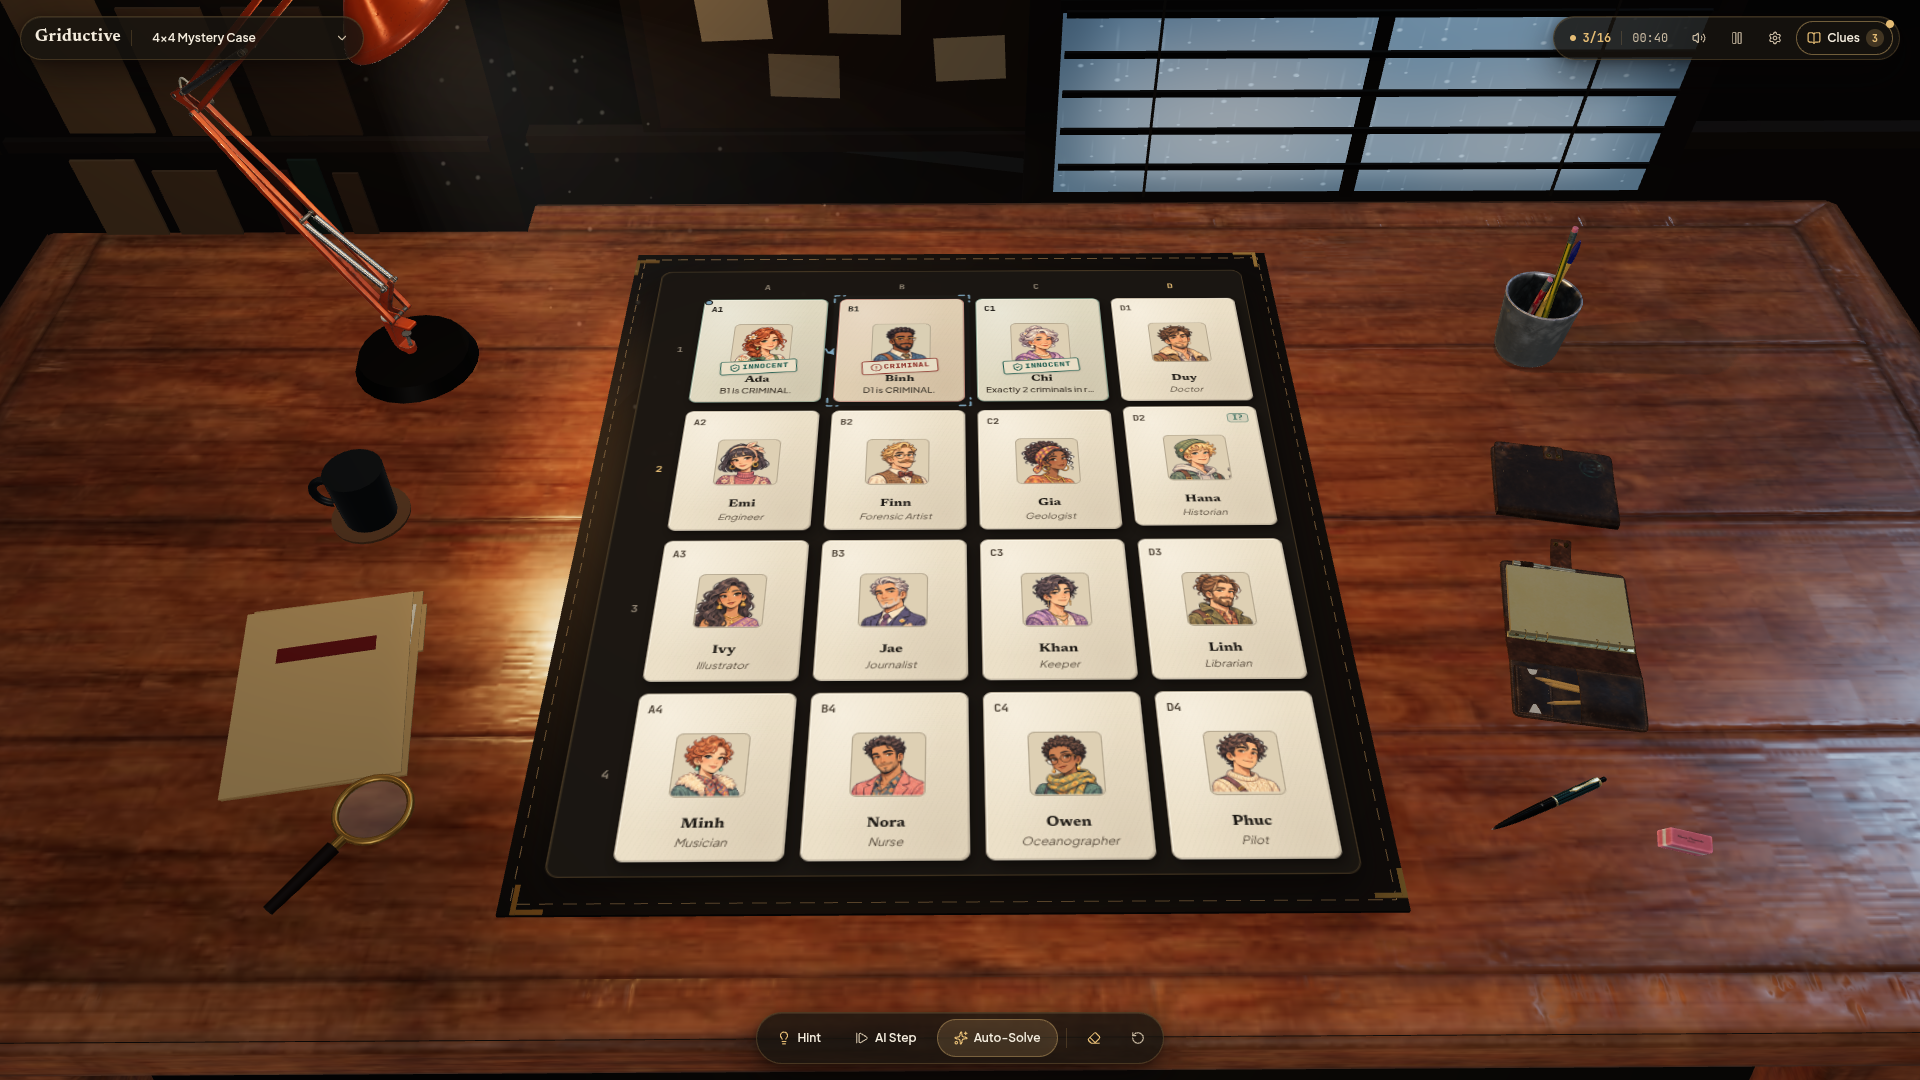
\includegraphics[width=0.92\textwidth]{images/gui_3d_overview.png}
    \caption{Không gian bàn điều tra ba chiều trên màn chơi $4 \times 4$ với các thẻ nghi phạm đã được đóng dấu xác nhận, đạo cụ thám tử và thanh công cụ hỗ trợ suy diễn tối giản}
    \label{fig:gui_overview}
\end{figure}

Để truyền tải trực quan triết lý suy diễn không đoán mò mà không làm gián đoạn mạch tư duy của người chơi bởi các hộp thoại cảnh báo rời rạc, mọi phản hồi logic đều được tích hợp trực tiếp lên bề mặt vật thể trong cảnh ba chiều. Cụ thể, khi người chơi chọn một lời khai trong ngăn kéo manh mối bên phải, hệ thống chiếu sáng trực tiếp đường viền của toàn bộ các thẻ nằm trong vùng không gian chịu sự chi phối của lời khai đó ngay trên mặt bàn. Đáng chú ý hơn, nếu người chơi nôn nóng đưa ra phán quyết cho một nghi phạm khi dữ kiện hiện tại chưa đủ sức chứng minh (chẳng hạn kết luận sớm về ô $\text{B2}$ khi mới chỉ biết một dữ kiện duy nhất tại hàng đầu tiên), một con dấu cao su màu hổ phách mang nhãn chưa thể chứng minh (\textit{``NOT PROVABLE''}) lập tức dập nghiêng trực tiếp xuống mặt thẻ ba chiều kèm hiệu ứng rung nhẹ rồi từ từ tan mực sau gần hai giây (Hình \ref{fig:gui_stamp_and_closed}a). Cuối cùng, khi toàn bộ các mắt xích trên bàn cờ đã được giải mã trọn vẹn, hồ sơ tổng kết vụ án xuất hiện chính giữa màn hình, cung cấp bức tranh định lượng minh bạch về số bước lập luận, tổng số truy vấn SAT, số phép lan truyền đơn vị, số lần quay lui và thời gian thực thi chính xác đến từng phần trăm mili-giây của bộ giải (Hình \ref{fig:gui_stamp_and_closed}b).

\begin{figure}[H]
    \centering
    \begin{subfigure}[t]{0.49\textwidth}
        \centering
        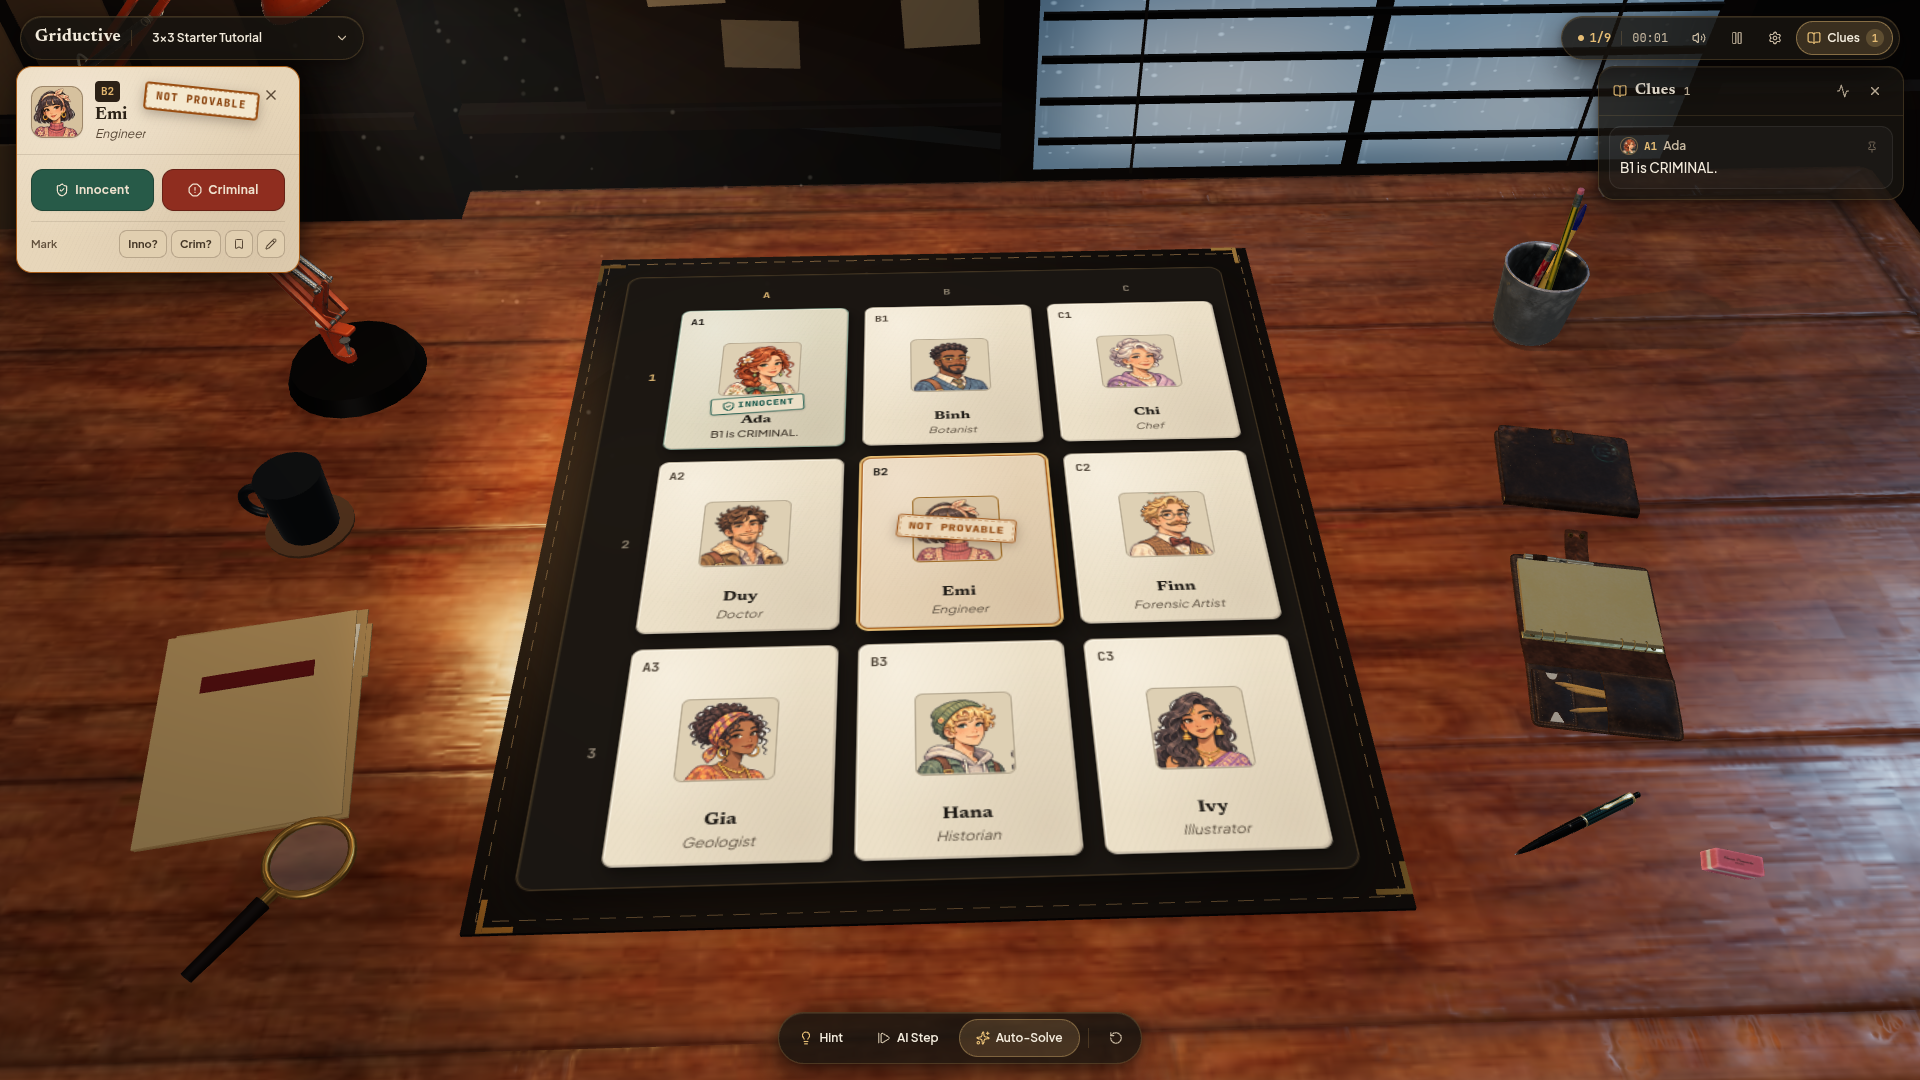
\includegraphics[width=\textwidth]{images/gui_not_provable_stamp.png}
        \caption{Hiệu ứng đóng dấu từ chối trực tiếp lên mặt thẻ $\text{B2}$ khi phán quyết chưa đủ cơ sở chứng minh}
        \label{fig:gui_stamp}
    \end{subfigure}
    \hfill
    \begin{subfigure}[t]{0.49\textwidth}
        \centering
        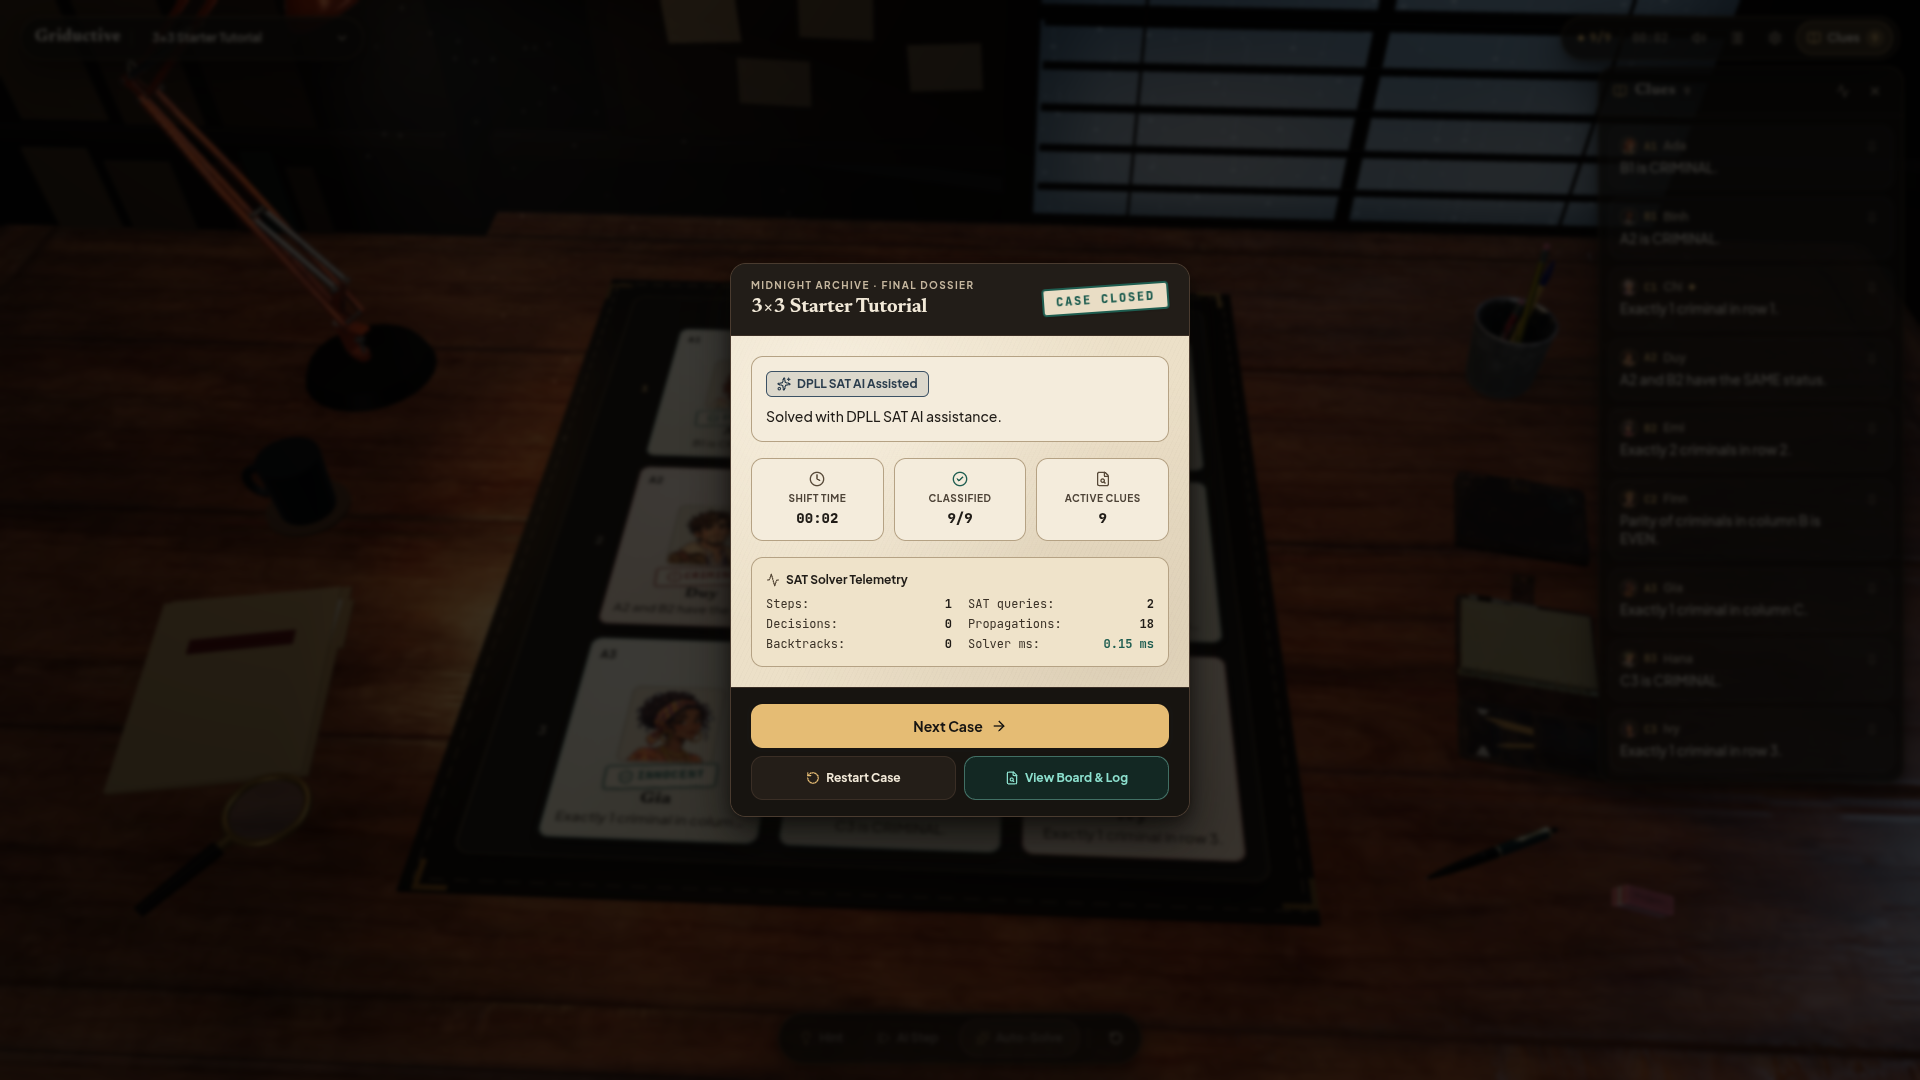
\includegraphics[width=\textwidth]{images/gui_case_closed.png}
        \caption{Hồ sơ khép lại vụ án hiển thị đầy đủ các chỉ số đo đạc vi mô của bộ giải mệnh đề}
        \label{fig:gui_closed}
    \end{subfigure}
    \caption{Phản hồi đóng dấu trực tiếp trên vật thể ba chiều và bảng thống kê thực thi sau khi hoàn tất suy diễn}
    \label{fig:gui_stamp_and_closed}
\end{figure}

\section{Biểu diễn tri thức và mã hóa CNF}
\label{sec:formulation}

Để một bộ giải thỏa mãn mệnh đề tổng quát có thể tự động lập luận trên các lời khai ngôn ngữ của trò chơi, toàn bộ cấu trúc không gian của bàn cờ và hệ thống quy tắc manh mối cần được chuyển dịch nhất quán sang ngôn ngữ logic mệnh đề ở dạng chuẩn hội (CNF). Chương này trình bày hệ thống ánh xạ biến song ánh, đại số tập hợp mô tả vùng không gian, bảng tổng hợp công thức mã hóa và các phép biến đổi tương đương đại số từng bước cho từng họ ràng buộc.

\subsection{Không gian biến mệnh đề}
\label{subsec:variable_mapping}
Xét bàn cờ vuông kích thước $N \times N$ được mô hình hóa thành lưới tọa độ nguyên rời rạc hai chiều $\mathcal{G}_N = \{(r, c) \in \mathbb{Z}^2 \mid 0 \le r < N,\; 0 \le c < N\}$ gồm đúng $N^2$ ô phân biệt, trong đó chỉ số hàng $r$ tăng từ trên xuống dưới và chỉ số cột $c$ tăng từ trái sang phải (tương ứng với cách đánh nhãn cột bằng chữ cái in hoa $\text{A}, \text{B}, \dots$ và hàng bằng số thứ tự $1, 2, \dots$ trên mặt bàn điều tra). Với mỗi vị trí $(r, c) \in \mathcal{G}_N$, ta định nghĩa một biến mệnh đề gốc $C_{r,c} \in \{\text{True}, \text{False}\}$ mang ý nghĩa quyết định thân phận của nghi phạm đứng tại ô đó: biến $C_{r,c}$ nhận chân trị $\text{True}$ khi và chỉ khi nghi phạm là tội phạm, và nhận chân trị $\text{False}$ khi và chỉ khi nghi phạm là người vô tội. Do thân phận của mỗi nhân vật mang tính nhị phân loại trừ lẫn nhau và hoàn toàn bất biến xuyên suốt ván đấu, tập hợp $N^2$ biến mệnh đề gốc này đủ để đặc tả trọn vẹn mọi cấu hình nghiệm khả dĩ của bàn cờ trong không gian trạng thái kích thước $2^{N^2}$.

Nhằm chuẩn hóa dữ liệu đầu vào cho bộ giải mệnh đề theo quy ước số nguyên khác không của chuẩn DIMACS (với số nguyên dương $+v$ biểu thị literal khẳng định $x_v$ và số nguyên âm $-v$ biểu thị literal phủ định $\neg x_v$), hệ thống thiết lập ánh xạ song ánh theo thứ tự ưu tiên hàng từ miền tọa độ hai chiều sang miền số nguyên dương liên tiếp:
\begin{equation}
    \phi_N : \mathcal{G}_N \to \{1, 2, \dots, N^2\}, \qquad \phi_N(r, c) = r \cdot N + c + 1
    \label{eq:var_map}
\end{equation}
đi kèm phép chiếu ngược duy nhất giúp khôi phục tọa độ lưới từ bất kỳ định danh biến gốc nào:
\begin{equation}
    \phi_N^{-1}(v) = \left(\left\lfloor \frac{v - 1}{N} \right\rfloor,\; (v - 1) \bmod N\right), \qquad \forall v \in \{1, 2, \dots, N^2\}.
\end{equation}
Bên cạnh tập biến gốc $V_{\text{gốc}} = \{1, 2, \dots, N^2\}$ gắn trực tiếp với các ô trên mặt bàn, một số phép biến đổi cấu trúc nâng cao như mạch chẵn lẻ tuyến tính cần sinh thêm các biến trung gian Tseitin để tránh bùng nổ số lượng mệnh đề \cite{tseitin1983complexity}. Các biến trung gian này được cấp phát tuần tự tăng dần bắt đầu từ $N^2 + 1$, tạo thành tập biến phụ trợ $V_{\text{phụ}} = \{N^2 + 1, N^2 + 2, \dots, N^2 + K\}$ rời nhau hoàn toàn với tập biến gốc ($V_{\text{gốc}} \cap V_{\text{phụ}} = \emptyset$). Cách phân hoạch không gian định danh chặt chẽ này vừa loại bỏ hoàn toàn nguy cơ đụng độ ký hiệu khi hợp nhất nhiều manh mối độc lập, vừa cho phép quy trình kiểm định nghiệm duy nhất chỉ cần xét sự biến thiên chân trị trên $V_{\text{gốc}}$ mà không bị phụ thuộc vào các biến trung gian nội bộ.

\subsection{Đại số vùng không gian}
\label{subsec:region_algebra}
Phần lớn các lời khai mang tính khái quát trong trò chơi không chỉ đích danh một cá nhân đơn lẻ mà áp đặt điều kiện định lượng lên một nhóm nghi phạm cùng chia sẻ thuộc tính vị trí trên lưới. Thay vì liệt kê thủ công từng ô cho mỗi loại manh mối, hệ thống xây dựng một đại số vùng hình học cho phép biểu diễn mọi miền tác động thông qua hàm phân giải tập hợp $\mathcal{R}_N(\cdot) \subseteq \mathcal{G}_N$ trả về danh sách các tọa độ không trùng lặp được sắp xếp chuẩn hóa theo thứ tự ưu tiên hàng. Ở cấp độ cơ sở, bốn miền hình học nguyên thủy bao gồm vùng hàng thứ $r_0$ được xác định bởi $\mathcal{R}_N(\text{Hàng}(r_0)) = \{(r_0, c) \mid 0 \le c < N\}$, vùng cột thứ $c_0$ được xác định bởi $\mathcal{R}_N(\text{Cột}(c_0)) = \{(r, c_0) \mid 0 \le r < N\}$, vùng liệt kê tường minh chứa một tập con tọa độ cho trước $S \subseteq \mathcal{G}_N$, và vùng lân cận tám hướng xung quanh tâm $(r_0, c_0)$ dựa trên khoảng cách Chebyshev bằng đơn vị (không tính bản thân ô tâm):
\begin{equation}
    \mathcal{R}_N(\text{LânCận}(r_0, c_0)) = \{(r, c) \in \mathcal{G}_N \mid \max(|r - r_0|,\, |c - c_0|) = 1\}.
\end{equation}
Tùy thuộc vào việc nhân vật làm tâm đứng ở bốn góc bàn cờ, nằm dọc theo rìa biên hay đứng hẳn bên trong lõi lưới, lực lượng của vùng lân cận tự động co giãn chính xác nhận các giá trị lần lượt bằng $3$, $5$ hoặc $8$ ô.

Không dừng lại ở các miền đơn lẻ, nhóm mở rộng đáng kể sức biểu đạt của ngôn ngữ lời khai thông qua phép toán \textbf{giao hai vùng bất kỳ} (phần mở rộng thứ nhất của hệ thống biểu diễn tri thức). Với hai biểu thức vùng thành phần $R_1$ và $R_2$, miền giao hợp thành được định nghĩa đệ quy bằng phép giao lý thuyết tập hợp $\mathcal{R}_N(\text{Giao}(R_1, R_2)) = \mathcal{R}_N(R_1) \cap \mathcal{R}_N(R_2)$ và tiếp tục bảo toàn thứ tự sắp xếp chuẩn hóa. Nhờ tính đóng của đại số tập hợp này, các phát biểu giao thoa không gian thường gặp trong các vụ án phức tạp --- chẳng hạn lời khai \textit{``Có đúng một tội phạm trong số những người vừa đứng ở hàng thứ hai vừa tiếp giáp trực tiếp với nghi phạm $\text{B1}$''} --- được rút gọn tự nhiên về một miền con xác định trước khi đưa vào bộ sinh mệnh đề, giúp tách bạch hoàn toàn bài toán hình học lưới khỏi bài toán biên dịch đại số Boole phía sau.

\subsection{Hệ thống manh mối và công thức CNF}
\label{subsec:clue_catalog}
Trên nền tảng biến mệnh đề và đại số vùng đã xác lập, hệ thống hỗ trợ đầy đủ sáu khuôn mẫu lời khai cốt lõi của trò chơi (gồm khẳng định đơn, đồng nhất trạng thái, đối lập trạng thái, tối thiểu $k$ tội phạm, tối đa $k$ tội phạm, và chính xác $k$ tội phạm) cùng khuôn mẫu mở rộng thứ hai là \textbf{ràng buộc tính chẵn lẻ số lượng tội phạm trên vùng} (chẵn hoặc lẻ). Bảng \ref{tab:cnf_catalog} tổng hợp bức tranh đối chiếu toàn diện giữa biểu thức ngữ nghĩa gốc, dạng chuẩn hội tương đương và quy mô số mệnh đề sinh ra theo kích thước vùng $m = |R|$.

\begin{table}[H]
\centering
\caption{Tổng hợp ngữ nghĩa toán học và công thức dạng chuẩn hội (CNF) cho sáu mẫu cốt lõi và mẫu mở rộng chẵn lẻ}
\label{tab:cnf_catalog}
\footnotesize
\begin{tabularx}{\textwidth}{l l >{\raggedright\arraybackslash}X r}
\toprule
\textbf{Họ manh mối} & \textbf{Biểu thức logic} & \textbf{Dạng chuẩn hội (CNF) tương đương} & \textbf{Số mệnh đề} \\
\midrule
Khẳng định tội phạm & $C_u$ & $(C_u)$ & $1$ \\
Khẳng định vô tội   & $\neg C_u$ & $(\neg C_u)$ & $1$ \\
\midrule
Đồng nhất trạng thái & $C_u \leftrightarrow C_v$ & $(\neg C_u \vee C_v) \wedge (C_u \vee \neg C_v)$ & $2$ \\
Đối lập trạng thái   & $C_u \oplus C_v$ & $(C_u \vee C_v) \wedge (\neg C_u \vee \neg C_v)$ & $2$ \\
\midrule
Tối thiểu $k$ tội phạm & $\sum_{x \in R} C_x \ge k$ & $\bigwedge_{S \in \binom{R}{m - k + 1}} \left(\bigvee_{x \in S} C_x\right)$ với $m = |R|$ & $\binom{m}{m-k+1}$ \\
Tối đa $k$ tội phạm    & $\sum_{x \in R} C_x \le k$ & $\bigwedge_{S \in \binom{R}{k + 1}} \left(\bigvee_{x \in S} \neg C_x\right)$ với $m = |R|$ & $\binom{m}{k+1}$ \\
Chính xác $k$ tội phạm & $\sum_{x \in R} C_x = k$ & Kết hợp hội của ràng buộc tối thiểu $k$ và tối đa $k$ trên cùng vùng $R$ & $\binom{m}{m-k+1} + \binom{m}{k+1}$ \\
\midrule
Chẵn lẻ vùng ($p \in \{0, 1\}$) & $\left(\sum_{x \in R} C_x\right) \bmod 2 = p$ & Chuỗi biến phụ $y_t \leftrightarrow (y_{t-1} \oplus C_{x_{t+1}})$ ghép với điều kiện khóa đuôi chẵn ($y_{m-2} \leftrightarrow C_{x_m}$) hoặc lẻ ($y_{m-2} \oplus C_{x_m}$) & $4m - 6$ \newline \scriptsize ($m \ge 2$) \\
\bottomrule
\end{tabularx}
\end{table}

\subsection{Biến đổi tương đương từng bước}
\label{subsec:step_by_step_derivations}

\subsubsection{Nhóm manh mối quan hệ nhị phân}
Đối với nhóm manh mối thiết lập sự phụ thuộc trực tiếp giữa hai nghi phạm phân biệt $u, v \in \mathcal{G}_N$ ($u \ne v$), quá trình chuyển đổi sang dạng chuẩn hội được dẫn xuất chặt chẽ bằng các luật tương đương cổ điển của đại số mệnh đề. Trước hết, xét lời khai đồng nhất khẳng định rằng $u$ và $v$ mang cùng thân phận, được biểu diễn bởi phép tương đương kép $C_u \leftrightarrow C_v$. Áp dụng lần lượt luật phân rã tương đương thành hội của hai phép kéo theo, luật khử phép kéo theo ($P \to Q \equiv \neg P \vee Q$) và tính giao hoán của phép tuyển, ta thu được biến đổi tương đương từng bước:
\begin{align}
    F_{\text{đồng nhất}}(u, v) &\equiv (C_u \leftrightarrow C_v) \nonumber\\
    &\equiv (C_u \to C_v) \wedge (C_v \to C_u) && \text{(Phân rã tương đương hai chiều)} \nonumber\\
    &\equiv (\neg C_u \vee C_v) \wedge (\neg C_v \vee C_u) && \text{(Khử phép kéo theo)} \nonumber\\
    &\equiv (\neg C_u \vee C_v) \wedge (C_u \vee \neg C_v). && \text{(Sắp xếp chuẩn hóa thứ tự biến)}
    \label{eq:cnf_same}
\end{align}
Chẳng hạn trên bàn cờ $3 \times 3$, lời khai khẳng định hai ô $\text{A2}$ và $\text{B2}$ cùng phe sẽ ánh xạ qua $\phi_3(\text{A2}) = 4$ và $\phi_3(\text{B2}) = 5$ thành hai mệnh đề bậc hai $(-4, 5)$ và $(4, -5)$. Ngay khi một trong hai ô được chứng minh mang một trạng thái cụ thể, một mệnh đề sẽ tự động thỏa mãn trong khi mệnh đề còn lại co về mệnh đề đơn vị, lập tức truyền trạng thái giống hệt sang ô kia.

Tiếp nối cách biến đổi trên, lời khai đối lập khẳng định $u$ và $v$ thuộc hai phe trái ngược nhau được biểu diễn thông qua phép tuyển loại trừ $C_u \oplus C_v \equiv (C_u \wedge \neg C_v) \vee (\neg C_u \wedge C_v)$. Để đưa biểu thức dạng chuẩn tuyển này về dạng chuẩn hội, ta áp dụng luật phân phối của phép tuyển đối với phép hội kết hợp luật bài trung ($P \vee \neg P \equiv \top$):
\begin{align}
    F_{\text{đối lập}}(u, v) &\equiv (C_u \wedge \neg C_v) \vee (\neg C_u \wedge C_v) \nonumber\\
    &\equiv \big((C_u \wedge \neg C_v) \vee \neg C_u\big) \wedge \big((C_u \wedge \neg C_v) \vee C_v\big) & \text{\footnotesize (Phân phối lần 1)} \nonumber\\
    &\equiv (C_u \vee \neg C_u) \wedge (\neg C_v \vee \neg C_u) \wedge (C_u \vee C_v) \wedge (\neg C_v \vee C_v) & \text{\footnotesize (Phân phối lần 2)} \nonumber\\
    &\equiv \top \wedge (\neg C_u \vee \neg C_v) \wedge (C_u \vee C_v) \wedge \top & \text{\footnotesize (Luật bài trung)} \nonumber\\
    &\equiv (C_u \vee C_v) \wedge (\neg C_u \vee \neg C_v).
    \label{eq:cnf_diff}
\end{align}
Hai mệnh đề thu được phản ánh trực quan hai mặt của sự đối lập: mệnh đề $(C_u \vee C_v)$ buộc ít nhất một trong hai người phải là tội phạm, trong khi mệnh đề $(\neg C_u \vee \neg C_v)$ ngăn không cho cả hai đồng thời là tội phạm.

\subsubsection{Nhóm manh mối đếm lực lượng vùng}
Chuyển sang nhóm manh mối định lượng trên vùng $R = \{x_1, x_2, \dots, x_m\}$ gồm $m = |R|$ ô phân biệt với ngưỡng nguyên không âm $k \ge 0$, nguyên lý biên dịch sang dạng chuẩn hội dựa trên việc loại trừ mọi tập con nhỏ nhất gây vi phạm ngưỡng đếm. Đối với ràng buộc cận trên yêu cầu có tối đa $k$ tội phạm trong vùng $R$, một phép gán chân trị vi phạm điều kiện này khi và chỉ khi tồn tại ít nhất một tập con $S \subseteq R$ gồm đúng $k + 1$ phần tử mà mọi biến trong $S$ đều đồng thời nhận giá trị $\text{True}$. Gọi $\binom{R}{k+1}$ là họ tất cả các tập con kích thước $k + 1$ trích ra từ $R$, phép phủ định điều kiện vi phạm kết hợp định luật De Morgan tổng quát cho ta chuỗi biến đổi tương đương:
\begin{align}
    \sum_{i=1}^{m} \mathbb{I}[C_{x_i}] \le k
    &\iff \neg \left( \bigvee_{S \in \binom{R}{k+1}} \bigwedge_{x \in S} C_x \right) && \text{(Cấm mọi tổ hợp $k+1$ tội phạm)} \nonumber\\
    &\iff \bigwedge_{S \in \binom{R}{k+1}} \neg \left( \bigwedge_{x \in S} C_x \right) && \text{(Định luật De Morgan ngoài)} \nonumber\\
    &\iff \bigwedge_{S \in \binom{R}{k+1}} \left( \bigvee_{x \in S} \neg C_x \right). && \text{(Định luật De Morgan trong)}
    \label{eq:at_most_cnf}
\end{align}
Bằng lập luận đối ngẫu hoàn toàn tương tự, yêu cầu có tối thiểu $k$ tội phạm trong vùng $m$ ô tương đương logic với việc có tối đa $m - k$ người vô tội trong vùng đó, tức $\sum_{i=1}^{m} \mathbb{I}[\neg C_{x_i}] \le m - k$. Thay thế mỗi biến $C_x$ bởi $\neg C_x$ và thay ngưỡng $k$ bởi $m - k$ vào Phương trình \eqref{eq:at_most_cnf} rồi rút gọn phủ định kép $\neg(\neg C_x) \equiv C_x$, ta dẫn xuất được công thức cận dưới gồm $\binom{m}{m-k+1}$ mệnh đề toàn dương:
\begin{equation}
    \sum_{i=1}^{m} \mathbb{I}[C_{x_i}] \ge k \iff \bigwedge_{S \in \binom{R}{m-k+1}} \left( \bigvee_{x \in S} C_x \right).
    \label{eq:at_least_cnf}
\end{equation}
Các trường hợp biên suy biến cũng được định nghĩa nhất quán về mặt toán học: ở cận trên, nếu $k \ge m$ thì điều kiện hiển nhiên đúng nên sinh ra tập mệnh đề rỗng, còn nếu $k = 0$ thì công thức sinh ra $m$ mệnh đề đơn vị $(\neg C_{x_1}) \wedge \dots \wedge (\neg C_{x_m})$; ngược lại ở cận dưới, nếu $k = 0$ thì công thức hiển nhiên đúng, còn nếu $k > m$ (đòi hỏi nhiều tội phạm hơn tổng số ghế trong vùng) thì công thức bất khả thỏa và sinh ra mệnh đề rỗng $\square$ để báo hiệu mâu thuẫn tức thời.

Để minh họa cụ thể cơ chế vận hành của phép biên dịch đếm lực lượng, xét lời khai \textit{``Có chính xác $2$ tội phạm ở hàng thứ nhất''} trên bàn cờ $4 \times 4$. Hàng đầu tiên bao gồm $m = 4$ ô $\{\text{A1}, \text{B1}, \text{C1}, \text{D1}\}$, được ánh xạ qua Phương trình \eqref{eq:var_map} thành tập biến $R = \{1, 2, 3, 4\}$ với ngưỡng $k = 2$. Ở nhánh cận dưới ($\sum_{x \in R} C_x \ge 2$), kích thước tổ hợp bằng $m - k + 1 = 4 - 2 + 1 = 3$, tạo ra $\binom{4}{3} = 4$ mệnh đề dương bậc ba:
\begin{equation}
    (C_1 \vee C_2 \vee C_3) \;\wedge\; (C_1 \vee C_2 \vee C_4) \;\wedge\; (C_1 \vee C_3 \vee C_4) \;\wedge\; (C_2 \vee C_3 \vee C_4).
\end{equation}
Song song đó, ở nhánh cận trên ($\sum_{x \in R} C_x \le 2$), kích thước tổ hợp bằng $k + 1 = 2 + 1 = 3$, tạo ra thêm $\binom{4}{3} = 4$ mệnh đề âm bậc ba:
\begin{equation}
    (\neg C_1 \vee \neg C_2 \vee \neg C_3) \;\wedge\; (\neg C_1 \vee \neg C_2 \vee \neg C_4) \;\wedge\; (\neg C_1 \vee \neg C_3 \vee \neg C_4) \;\wedge\; (\neg C_2 \vee \neg C_3 \vee \neg C_4).
\end{equation}
Khi hợp nhất hai nhánh lại, lời khai được biểu diễn trọn vẹn bởi đúng $8$ mệnh đề bậc ba. Giả sử ở các bước tiếp theo, hai nghi phạm $\text{B1}$ ($C_2 = \text{True}$) và $\text{D1}$ ($C_4 = \text{True}$) được xác định là tội phạm; khi đó hai mệnh đề âm $(\neg C_1 \vee \neg C_2 \vee \neg C_4)$ và $(\neg C_2 \vee \neg C_3 \vee \neg C_4)$ lập tức bị rút gọn bởi cơ chế lan truyền đơn vị thành hai mệnh đề đơn $(\neg C_1)$ và $(\neg C_3)$, buộc cả $\text{A1}$ lẫn $\text{C1}$ phải là người vô tội mà không cần bất kỳ thao tác đoán thử nào.

\subsubsection{Nhóm manh mối mở rộng tính chẵn lẻ bằng chuỗi XOR tuyến tính}
\label{subsubsec:parity_cnf}
Khác với các ràng buộc ngưỡng đơn điệu, lời khai tính chẵn lẻ trên vùng $R = \{x_1, \dots, x_m\}$ đòi hỏi tổng số tội phạm chia cho $2$ có số dư cố định bằng $0$ (chẵn) hoặc bằng $1$ (lẻ), tức biểu thức chuỗi tuyển loại trừ $C_{x_1} \oplus C_{x_2} \oplus \dots \oplus C_{x_m}$ phải nhận chân trị $\text{False}$ (nếu chẵn) hoặc $\text{True}$ (nếu lẻ). Nếu áp dụng cách khai triển bảng chân trị trực tiếp chỉ dùng các biến gốc $C_{x_i}$, mỗi phép gán sai tính chẵn lẻ trong tổng số $2^m$ tổ hợp đòi hỏi đúng một mệnh đề độ rộng $m$ để loại bỏ, dẫn tới số lượng mệnh đề tăng vọt theo hàm mũ $2^{m-1}$ (lên tới $32.768$ mệnh đề khi $m = 16$).

Nhằm triệt tiêu sự bùng nổ hàm mũ này đối với mọi vùng có kích thước $m \ge 3$, nhóm triển khai kỹ thuật phân rã dây chuyền Tseitin \cite{tseitin1983complexity} bằng cách đưa vào $m - 2$ biến phụ trợ $y_1, y_2, \dots, y_{m-2} \in V_{\text{phụ}}$ đóng vai trò thanh ghi cộng dồn tính lẻ của các tiền tố liên tiếp:
\begin{equation}
    y_1 \leftrightarrow (C_{x_1} \oplus C_{x_2}), \qquad
    y_t \leftrightarrow (y_{t-1} \oplus C_{x_{t+1}}) \quad \forall t \in \{2, \dots, m - 2\}.
\end{equation}
Xét một mắt xích cơ sở tổng quát $z \leftrightarrow (a \oplus b)$, áp dụng định nghĩa tương đương hai chiều và biến đổi đại số từng bước sang dạng chuẩn hội:
\begin{align}
    z \leftrightarrow (a \oplus b)
    &\equiv \big(z \to (a \oplus b)\big) \wedge \big((a \oplus b) \to z\big) \nonumber\\
    &\equiv \big(\neg z \vee ((a \vee b) \wedge (\neg a \vee \neg b))\big) \wedge \big(\neg((a \wedge \neg b) \vee (\neg a \wedge b)) \vee z\big) \nonumber\\
    &\equiv (\neg z \vee a \vee b) \wedge (\neg z \vee \neg a \vee \neg b) \wedge \big(((\neg a \vee b) \wedge (a \vee \neg b)) \vee z\big) \nonumber\\
    &\equiv (a \vee b \vee \neg z) \wedge (\neg a \vee \neg b \vee \neg z) \wedge (\neg a \vee b \vee z) \wedge (a \vee \neg b \vee z).
    \label{eq:xor_gate_cnf}
\end{align}
Như vậy, mỗi mắt xích trung gian luôn tiêu tốn cố định đúng $4$ mệnh đề bậc ba bất kể chuỗi dài bao nhiêu. Tại mắt xích khóa đuôi cuối cùng kết nối biến tích lũy $y_{m-2}$ với biến gốc cuối cùng $C_{x_m}$, nếu lời khai yêu cầu tổng lẻ thì $y_{m-2} \oplus C_{x_m}$ được biên dịch theo Phương trình \eqref{eq:cnf_diff} thành hai mệnh đề $(y_{m-2} \vee C_{x_m}) \wedge (\neg y_{m-2} \vee \neg C_{x_m})$; ngược lại, nếu lời khai yêu cầu tổng chẵn thì điều kiện $y_{m-2} \leftrightarrow C_{x_m}$ được biên dịch theo Phương trình \eqref{eq:cnf_same} thành hai mệnh đề $(\neg y_{m-2} \vee C_{x_m}) \wedge (y_{m-2} \vee \neg C_{x_m})$. Cộng gộp toàn chuỗi với $m \ge 2$, phương pháp mã hóa chỉ phát sinh đúng $4(m - 2) + 2 = 4m - 6$ mệnh đề có độ rộng tối đa bằng $3$, bảo đảm tính thỏa mãn tương đương (\textit{equisatisfiability}) với độ phức tạp không gian tuyến tính tuyệt đối $\Theta(m)$.

\subsection{Hợp nhất và kiểm chứng tri thức}
\label{subsec:kb_assembly}
Tại mỗi bước suy diễn thứ $t$, từ bản chụp công khai chứa tập các ô đã mở (cùng trạng thái tội phạm hoặc vô tội đã biết của chúng) và tập các lời khai hiện hữu $\mathcal{C}_t$, cơ sở tri thức tổng thể $KB_t$ được kiến tạo bằng phép hội của toàn bộ các mệnh đề đơn vị phản ánh thân phận đã biết với các khối mệnh đề biên dịch từ từng lời khai:
\begin{equation}
    KB_t \;=\; \bigwedge_{u \in \mathcal{K}_t^{+}} (C_u) \;\wedge\; \bigwedge_{v \in \mathcal{K}_t^{-}} (\neg C_v) \;\wedge\; \bigwedge_{c \in \mathcal{C}_t} \text{CNF}(c),
    \label{eq:kb_total}
\end{equation}
trong đó $\mathcal{K}_t^{+}$ và $\mathcal{K}_t^{-}$ lần lượt ký hiệu tập các ô đã được xác nhận là tội phạm và tập các ô đã được xác nhận là vô tội tính đến bước $t$. Trước khi chuyển giao cho bộ giải, toàn bộ các mệnh đề thành phần được đi qua quy trình chuẩn hóa ba tầng bảo toàn tương đương logic: khử các literal lặp lại bên trong cùng một mệnh đề, loại bỏ hoàn toàn các mệnh đề hằng đúng chứa đồng thời một biến và phủ định của chính nó, cuối cùng loại bỏ các mệnh đề trùng lặp xuất hiện giữa nhiều lời khai giao nhau mà vẫn giữ nguyên thứ tự xuất hiện tất định.

Nhằm kiểm chứng độc lập độ chính xác toán học của toàn bộ tầng mã hóa mà không phụ thuộc vào giả định đúng đắn của chính nó, nhóm xây dựng song song một bộ định giá ngữ nghĩa trực tiếp hoạt động bằng cách đếm số lượng và kiểm tra quan hệ chân trị nguyên bản trên từng cấu hình bàn cờ hoàn chỉnh. Thông qua phép thử vét cạn toàn bộ $2^{N^2}$ bảng phân bố chân trị trên lưới $3 \times 3$ ($512$ cấu hình) và lưới $4 \times 4$ ($65.536$ cấu hình), nhóm đã xác minh thực nghiệm rằng điều kiện đồng dư ngữ nghĩa sau đây luôn được thỏa mãn tuyệt đối cho mọi họ lời khai và mọi trường hợp biên:
\begin{equation}
    M_{\text{gốc}} \models_{\text{ngữ nghĩa}} c \iff \exists M_{\text{phụ}} : (M_{\text{gốc}} \cup M_{\text{phụ}}) \models_{\text{CNF}} \text{CNF}(c).
\end{equation}
Sự trùng khớp một--một giữa định giá ngữ nghĩa gốc và tập nghiệm chiếu trên biến gốc của công thức CNF là cơ sở vững chắc bảo đảm tác tử suy diễn không bao giờ mắc sai số biên dịch trong mọi tình huống phức tạp.

\section{Giải thuật suy diễn và bộ giải SAT}
\label{sec:algorithms}

Sau khi cơ sở tri thức công khai tại từng thời điểm đã được chuyển hóa thành tập mệnh đề chuẩn hội $KB_t$, bài toán cốt lõi tiếp theo là thiết kế cơ chế suy diễn tự động có khả năng tìm ra chính xác những ô bị ép buộc chân trị mà không bao giờ vi phạm nguyên tắc cấm đoán mò. Chương này trình bày chi tiết thuật toán giải thỏa mãn mệnh đề DPLL tự cài đặt, định lý suy diễn hệ quả bằng phản chứng, chứng minh toán học cho kỹ thuật bộ nhớ đệm mô hình chứng nhân và phương pháp kiểm định tính duy nhất của nghiệm.

\subsection{Giải thuật DPLL tất định}
\label{subsec:dpll_solver}
Bài toán kiểm tra tính thỏa được của một công thức logic mệnh đề ở dạng chuẩn hội (SAT) là bài toán $\text{NP}$-đầy đủ đầu tiên trong lịch sử khoa học máy tính \cite{cook1971complexity}. Thay vì dựa vào các thư viện tối ưu hóa đóng gói sẵn bên ngoài, nhóm tự thiết kế và hiện thực trọn vẹn giải thuật \textbf{Davis--Putnam--Logemann--Loveland (DPLL)} \cite{davis1960computing,davis1962machine} kết hợp cơ chế truyền danh sách giả định tạm thời, được trình bày hình thức trong Thuật toán \ref{alg:dpll}. Việc hỗ trợ danh sách giả định $\mathcal{A} = (\ell_1, \dots, \ell_q)$ ngay tại đầu vào cho phép tác tử suy diễn liên tục đặt các câu hỏi giả định ngược lên cùng một tập mệnh đề $KB_t$ bất biến mà không cần cấp phát lại hay làm xáo trộn cấu trúc cơ sở tri thức gốc.

\begin{algorithm}[H]
\caption{Giải thuật DPLL tất định kết hợp lan truyền mệnh đề đơn vị}
\label{alg:dpll}
\footnotesize
\begin{algorithmic}[1]
\Require Tập mệnh đề chuẩn hội $\mathcal{F}$, dãy literal giả định tạm thời $\mathcal{A}$
\Ensure Kết quả khả thỏa, mô hình chân trị $M$ (nếu có) và bộ thống kê thực thi
\State $V \gets \text{SắpXếpTăngDần}\big(\{|\ell| : C \in \mathcal{F}, \ell \in C\} \cup \{|\ell| : \ell \in \mathcal{A}\}\big)$
\State $\sigma_0 \gets \emptyset$; \quad $n_{\text{nhánh}} \gets 0$; \quad $n_{\text{lan truyền}} \gets 0$; \quad $n_{\text{quay lui}} \gets 0$
\For{mỗi literal $\ell \in \mathcal{A}$}
    \If{$|\ell| \in \text{miền}(\sigma_0)$ \textbf{và} $\sigma_0(|\ell|) \ne (\ell > 0)$}
        \State \Return $\langle \text{False},\; \varnothing,\; (n_{\text{nhánh}}, n_{\text{lan truyền}}, n_{\text{quay lui}}) \rangle$
    \EndIf
    \State $\sigma_0(|\ell|) \gets (\ell > 0)$
\EndFor
\Function{LanTruyềnĐơnVị}{$\mathcal{F}, \sigma$}
    \Loop
        \State $f \gets \text{False}$
        \For{mỗi mệnh đề $C \in \mathcal{F}$}
            \If{$\exists \ell \in C : |\ell| \in \text{miền}(\sigma) \wedge \sigma(|\ell|) = (\ell > 0)$}
                \State \textbf{continue}
            \EndIf
            \State $U \gets [\ell \in C \mid |\ell| \notin \text{miền}(\sigma)]$
            \If{$|U| = 0$}
                \State \Return $\bot$ \Comment{Xung đột: mọi literal trong mệnh đề $C$ đều nhận chân trị sai}
            \ElsIf{$|U| = 1$}
                \State $\ell^* \gets U[0]$; \quad $\sigma(|\ell^*|) \gets (\ell^* > 0)$
                \State $n_{\text{lan truyền}} \gets n_{\text{lan truyền}} + 1$; \quad $f \gets \text{True}$; \quad \textbf{break}
            \EndIf
        \EndFor
        \If{$\neg f$} \Return $\sigma$ \EndIf
    \EndLoop
\EndFunction
\Function{DuyệtNhánh}{$\mathcal{F}, \sigma$}
    \State $\sigma' \gets \Call{LanTruyềnĐơnVị}{\mathcal{F}, \sigma}$
    \If{$\sigma' = \bot$} \Return $\bot$ \EndIf
    \If{mọi mệnh đề $C \in \mathcal{F}$ đều đã có ít nhất một literal đúng dưới $\sigma'$} \Return $\sigma'$ \EndIf
    \State $v^* \gets \min \{v \in V \mid v \notin \text{miền}(\sigma')\}$
    \For{$b \in (\text{True}, \text{False})$}
        \State $n_{\text{nhánh}} \gets n_{\text{nhánh}} + 1$
        \State $\sigma_{\text{mới}} \gets \text{BảnSao}(\sigma')$; \quad $\sigma_{\text{mới}}(v^*) \gets b$
        \State $\tau \gets \Call{DuyệtNhánh}{\mathcal{F}, \sigma_{\text{mới}}}$
        \If{$\tau \ne \bot$} \Return $\tau$ \EndIf
        \State $n_{\text{quay lui}} \gets n_{\text{quay lui}} + 1$
    \EndFor
    \State \Return $\bot$
\EndFunction
\State $\sigma^* \gets \Call{DuyệtNhánh}{\mathcal{F}, \sigma_0}$
\If{$\sigma^* = \bot$} \Return $\langle \text{False},\; \varnothing,\; (n_{\text{nhánh}}, n_{\text{lan truyền}}, n_{\text{quay lui}}) \rangle$ \EndIf
\State $M \gets \{v \mapsto \sigma^*(v) \text{ nếu } v \in \text{miền}(\sigma^*) \text{ ngược lại } \text{False} \mid v \in V\}$
\State \Return $\langle \text{True},\; M,\; (n_{\text{nhánh}}, n_{\text{lan truyền}}, n_{\text{quay lui}}) \rangle$
\end{algorithmic}
\end{algorithm}

Động cơ cắt tỉa mạnh mẽ nhất bên trong giải thuật trên chính là thủ tục \textbf{lan truyền mệnh đề đơn vị lặp đến điểm bất động}. Xét dưới một phép gán chân trị một phần $\sigma$, nếu một mệnh đề $C$ chưa được thỏa mãn và toàn bộ các literal trong $C$ ngoại trừ duy nhất một literal chưa gán $\ell^*$ đều đã bị gán giá trị sai, thì $\ell^*$ bắt buộc phải nhận giá trị đúng để duy trì khả năng thỏa mãn của $C$. Mỗi phép ép buộc như vậy lại tiếp tục làm co ngắn các mệnh đề liên đới khác và có thể nhanh chóng làm lộ diện mệnh đề rỗng ($|U| = 0$) khi xảy ra mâu thuẫn dây chuyền. Chỉ khi quá trình lan truyền đạt tới trạng thái bão hòa mà công thức vẫn chưa thỏa hết, bộ giải mới chọn biến chưa gán có chỉ số nhỏ nhất $v^* \in V$ để thử lần lượt hai nhánh $\text{True}$ rồi $\text{False}$ trên bản sao trạng thái độc lập. Nhờ quy tắc chọn biến cố định này, cây tìm kiếm hoàn toàn tất định và tái lập chính xác mọi thông số đo đạc trên mọi máy tính. Về mặt độ phức tạp, với $V$ biến và tổng độ dài xuất hiện literal bằng $L = \sum_{C \in \mathcal{F}} |C|$, mỗi pha lan truyền đến điểm bất động tốn tối đa $O(V \cdot L)$ phép kiểm tra; trong trường hợp xấu nhất trên các công thức đối xứng vô nghiệm, thời gian chạy bị chặn trên bởi $O(2^V \cdot V \cdot L)$ với chi phí bộ nhớ ngăn xếp đệ quy đa thức $O(V^2)$.

\subsection{Suy diễn hệ quả bằng phản chứng}
\label{subsec:logic_agent}
Khác với bài toán tìm một nghiệm bất kỳ, nhiệm vụ của tác tử suy diễn tại bước $t$ là chứng minh xem liệu một biến gốc $C_i$ (ứng với ô chưa mở $i$) có mang cùng một chân trị duy nhất trên \textit{mọi} mô hình của $KB_t$ hay không. Nền tảng toán học chuyển đổi bài toán kiểm tra hệ quả logic sang bài toán kiểm tra tính bất khả thỏa được phát biểu qua định lý phản chứng kinh điển sau đây \cite{russell2020aima}.

\noindent\textbf{Định lý 1 (Kiểm định hệ quả mệnh đề bằng phản chứng):}
\textit{Cho cơ sở tri thức mệnh đề $KB_t$ và một literal đơn $\ell \in \{C_i, \neg C_i\}$. Khi đó $KB_t$ kéo theo logic $\ell$ ($KB_t \models \ell$) khi và chỉ khi công thức mở rộng $KB_t \wedge \neg \ell$ là không thỏa được.}

\noindent\textbf{Chứng minh:}
Theo định nghĩa ngữ nghĩa chuẩn của quan hệ hệ quả logic, $KB_t \models \ell$ xảy ra khi và chỉ khi với mọi phép gán chân trị $M$, nếu $M$ làm thỏa toàn bộ các mệnh đề trong $KB_t$ ($M \models KB_t$) thì $M$ cũng đồng thời làm thỏa $\ell$ ($M \models \ell$). Phát biểu này tương đương logic với mệnh đề phủ định rằng không tồn tại bất kỳ phép gán $M$ nào làm thỏa $KB_t$ nhưng lại làm sai $\ell$ (tức làm đúng $\neg \ell$). Nói cách khác, tập hợp mô hình của công thức hội $\text{MôHình}(KB_t \wedge \neg \ell) = \emptyset$, đồng nghĩa $KB_t \wedge \neg \ell$ là không thỏa được. $\blacksquare$

Mặc dù Định lý 1 cho phép chứng minh một chiều, việc chỉ thực hiện một phép thử đơn lẻ sẽ gặp bẫy logic nếu bản thân $KB_t$ chứa dữ liệu mâu thuẫn nội tại ($\text{MôHình}(KB_t) = \emptyset$), bởi khi đó nguyên lý bùng nổ khiến cả $KB_t \wedge \neg C_i$ lẫn $KB_t \wedge C_i$ đều đồng thời không thỏa được. Để bảo đảm an toàn tuyệt đối trước cả các tập dữ liệu lỗi, tác tử suy diễn đánh giá đầy đủ cặp kết quả khả thỏa dưới giả định phủ định $S^- = \text{KhảThỏa}(KB_t \wedge \neg C_i)$ và dưới giả định khẳng định $S^+ = \text{KhảThỏa}(KB_t \wedge C_i)$, từ đó phân loại chính xác từng ô chưa mở vào đúng một trong bốn phạm trù rời nhau trong Bảng \ref{tab:entailment_truth_table}.

\begin{table}[H]
\centering
\caption{Ma trận phân loại suy diễn bốn trạng thái cho ô $i$ dựa trên cặp truy vấn giả định ngược}
\label{tab:entailment_truth_table}
\footnotesize
\setlength{\tabcolsep}{5pt}
\begin{tabularx}{\textwidth}{c c l >{\raggedright\arraybackslash}X}
\toprule
$\text{KhảThỏa}(KB_t \wedge \neg C_i)$ & $\text{KhảThỏa}(KB_t \wedge C_i)$ & \textbf{Kết luận phân loại} & \textbf{Diễn giải ngữ nghĩa hình thức} \\
\midrule
Không thỏa & Thỏa được  & \textbf{Tội phạm}       & $KB_t$ nhất quán và mọi mô hình của $KB_t$ đều buộc $C_i = \text{True}$. \\
Thỏa được  & Không thỏa & \textbf{Vô tội}         & $KB_t$ nhất quán và mọi mô hình của $KB_t$ đều buộc $C_i = \text{False}$. \\
Thỏa được  & Thỏa được  & \textbf{Chưa xác định}  & Tồn tại cả mô hình tội phạm lẫn mô hình vô tội; mọi phán quyết đều là đoán mò. \\
Không thỏa & Không thỏa & \textbf{Mâu thuẫn}      & Tập manh mối hiện hành vô nghiệm ($\text{MôHình}(KB_t) = \emptyset$). \\
\bottomrule
\end{tabularx}
\end{table}

\subsection{Bộ nhớ đệm mô hình chứng nhân}
\label{subsec:witness_cache}
Nếu áp dụng trực tiếp Bảng \ref{tab:entailment_truth_table} một cách máy móc cho từng ô trong tập các ô chưa mở $U_t$, mỗi ô chưa đủ dữ kiện để kết luận luôn tiêu tốn hai lượt gọi bộ giải DPLL độc lập, đẩy tổng chi phí mỗi bước lên tới $2|U_t|$ truy vấn. Tuy nhiên, nhóm nhận thấy rằng mỗi khi một lượt gọi DPLL kết thúc với trạng thái thỏa được, nghiệm trả về $M$ không chỉ chứng thực riêng cho một biến đang xét mà thực chất là một \textbf{mô hình chứng nhân toàn cục} thỏa mãn đồng thời toàn bộ $KB_t$. Từ nhận thức này, nhóm đề xuất kỹ thuật lưu đệm các mô hình chứng nhân thu thập được ngay trong nội bộ bước $t$ để cắt tỉa sớm các truy vấn dư thừa trên những ô kế tiếp.

\noindent\textbf{Mệnh đề 2 (Tính đúng đắn của bộ nhớ đệm mô hình chứng nhân theo bước):}
\textit{Xét tại một bước suy diễn cố định $t$ với cơ sở tri thức $KB_t$, giả sử tập mô hình chứng nhân $\mathcal{W}_t$ lưu giữ các mô hình $M$ sinh ra từ những lượt gọi DPLL thỏa được trước đó trong cùng bước $t$. Với mọi ô chưa mở $j \in U_t$ có biến mệnh đề tương ứng $v_j = \phi_N(j)$ nằm trong miền xác định của một mô hình $M \in \mathcal{W}_t$: nếu $M(v_j) = \text{True}$ thì công thức $KB_t \wedge C_j$ chắc chắn thỏa được mà không cần gọi lại bộ giải; tương tự, nếu $M(v_j) = \text{False}$ thì công thức $KB_t \wedge \neg C_j$ chắc chắn thỏa được.}

\noindent\textbf{Chứng minh:}
Mỗi mô hình $M \in \mathcal{W}_t$ là đầu ra hợp lệ của giải thuật DPLL trên tập mệnh đề $KB_t$ kết hợp một giả định phụ nào đó $\mathcal{A}$, nghĩa là $M \models (KB_t \wedge \bigwedge_{\ell \in \mathcal{A}} \ell)$, suy ra tất yếu $M \models KB_t$. Khi biến $v_j$ thuộc miền xác định của $M$ và nhận giá trị $M(v_j) = \text{True}$, phép gán $M$ hiển nhiên làm đúng đồng thời cả $KB_t$ lẫn mệnh đề đơn $(C_j)$, chứng tỏ $\text{MôHình}(KB_t \wedge C_j) \ne \emptyset$. Lập luận hoàn toàn đối xứng cho trường hợp $M(v_j) = \text{False}$ kéo theo $M \models (KB_t \wedge \neg C_j)$. Đáng lưu ý, đối với những ô cô lập chưa từng xuất hiện trong bất kỳ lời khai nào của $KB_t$ ($v_j \notin \text{miền}(M)$), phép tra cứu chứng nhân trả về kết quả chưa được chứng kiến để buộc bộ giải thực hiện kiểm tra chuẩn xác, nhờ đó bảo toàn tính đúng đắn và tính đầy đủ $100\%$ so với phương pháp phản chứng gốc. $\blacksquare$

Một chi tiết thiết kế sống còn bảo đảm tính toàn vẹn của cơ chế trên là \textbf{vòng đời của bộ nhớ đệm $\mathcal{W}_t$ bị giới hạn nghiêm ngặt trong phạm vi duy nhất một bước $t$}. Ngay khi tác tử tìm ra một ô bị ép buộc và mở thẻ để nhận thêm lời khai mới $c_{\text{mới}}$, cơ sở tri thức chuyển sang bước kế tiếp $KB_{t+1} = KB_t \wedge (\ell^*) \wedge \text{CNF}(c_{\text{mới}})$. Do tính chất đơn điệu của logic mệnh đề làm co hẹp không gian nghiệm $\text{MôHình}(KB_{t+1}) \subseteq \text{MôHình}(KB_t)$, các mô hình cũ trong $\mathcal{W}_t$ rất có thể vi phạm lời khai mới $c_{\text{mới}}$ và không còn hợp lệ ở bước $t + 1$. Chính vì vậy, việc khởi tạo mới hoàn toàn tập chứng nhân ở đầu mỗi chu kỳ quét giúp hệ thống vừa khai thác tối đa thông tin từ các mô hình đã giải, vừa miễn nhiễm tuyệt đối trước lỗi dùng lại chứng nhân lỗi thời.

\subsection{Chu trình giải tự động và nghiệm duy nhất}
\label{subsec:auto_loop_uniqueness}
Kết hợp trọn vẹn các thành phần trên, chu trình suy diễn tự động toàn cục của tác tử được trình bày trong Thuật toán \ref{alg:logic_loop}. Ở từng vòng lặp, tác tử trích xuất trạng thái công khai mới nhất, biên dịch $KB_t$, khởi tạo tập chứng nhân rỗng $\mathcal{W}_t$ và duyệt tuần tự các ô chưa mở theo đúng thứ tự ưu tiên hàng ($\text{A1}, \text{B1}, \dots$). Ngay khi bắt gặp ô đầu tiên có một chiều giả định bị bác bỏ (chứng tỏ chiều ngược lại bị ép buộc tất yếu), tác tử lập tức dừng quét bước hiện tại, gửi phán quyết kèm chỉ số phiên bản để lật mở dữ kiện mới và lặp lại chu trình. Trái lại, nếu đã quét hết toàn bộ các ô chưa mở mà mọi ô đều rơi vào trạng thái chưa xác định, vòng lặp chủ động dừng lại an toàn và báo cáo trạng thái bế tắc do đa nghiệm thay vì liều lĩnh chọn bừa một nhánh.

\begin{algorithm}[H]
\caption{Chu trình suy diễn tự động nghiêm ngặt không đoán mò}
\label{alg:logic_loop}
\footnotesize
\begin{algorithmic}[1]
\Require Môi trường quản trị ván đấu cung cấp bản chụp công khai và giao thức mở thẻ
\Ensure Trạng thái kết thúc cùng hồ sơ vết suy diễn và thông số tích lũy qua từng bước
\While{bàn cờ vẫn còn ô chưa được mở}
    \If{thời gian thực thi vượt ngưỡng giới hạn cho phép} \Return \text{QuáHạnThờiGian} \EndIf
    \State Trích xuất bản chụp trạng thái công khai $S_t$ và biên dịch cơ sở tri thức $KB_t$
    \State $U_t \gets \text{SắpXếpƯuTiênHàng}(\text{CácÔChưaMở}(S_t))$; \quad $\mathcal{W}_t \gets \emptyset$
    \State $u^* \gets \varnothing$; \quad $s^* \gets \varnothing$
    \For{mỗi ô $u \in U_t$ có mã biến $v = \phi_N(u)$}
        \If{$\exists M \in \mathcal{W}_t : v \in \text{miền}(M) \wedge M(v) = \text{False}$}
            \State $S^- \gets \text{True}$
        \Else
            \State $\langle S^-, M^- \rangle \gets \text{DPLL}(KB_t,\; (-v))$
            \If{$S^-$} $\mathcal{W}_t \gets \mathcal{W}_t \cup \{M^-\}$ \EndIf
        \EndIf
        \If{$\exists M \in \mathcal{W}_t : v \in \text{miền}(M) \wedge M(v) = \text{True}$}
            \State $S^+ \gets \text{True}$
        \Else
            \State $\langle S^+, M^+ \rangle \gets \text{DPLL}(KB_t,\; (+v))$
            \If{$S^+$} $\mathcal{W}_t \gets \mathcal{W}_t \cup \{M^+\}$ \EndIf
        \EndIf
        \If{$\neg S^- \wedge \neg S^+$} \Return \text{MâuThuẫnTriThức} \EndIf
        \If{$\neg S^- \wedge S^+$}
            \State $\langle u^*, s^* \rangle \gets \langle u, \text{TộiPhạm} \rangle$; \quad \textbf{break}
        \ElsIf{$S^- \wedge \neg S^+$}
            \State $\langle u^*, s^* \rangle \gets \langle u, \text{VôTội} \rangle$; \quad \textbf{break}
        \EndIf
    \EndFor
    \If{$u^* = \varnothing$}
        \State \Return \text{DừngDoĐaNghiệm} \Comment{Tuyệt đối không suy đoán khi chưa đủ dữ kiện}
    \EndIf
    \State Xác nhận phán quyết $\langle u^*, s^* \rangle$ để mở lời khai kế tiếp và ghi vết bước giải
\EndWhile
\State \Return \text{GiảiHoànTất}
\end{algorithmic}
\end{algorithm}

Bên cạnh bài toán giải tuần tự theo tiến trình mở thẻ, hệ thống còn cung cấp quy trình \textbf{kiểm định tính duy nhất của nghiệm} trên toàn bộ lời khai của màn chơi nhằm thẩm định tính chặt chẽ của thiết kế câu đố chỉ với đúng hai lượt gọi bộ giải DPLL. Ở lượt thứ nhất, toàn bộ các lời khai cùng các ô mở sẵn ban đầu được mã hóa thành công thức $KB_{\text{toàn phần}}$ (tuyệt đối không đưa đáp án ẩn vào) để tìm nghiệm khả thỏa đầu tiên $M_1$. Nếu $KB_{\text{toàn phần}}$ vô nghiệm hoặc tồn tại bất kỳ biến gốc $v \in V_{\text{gốc}}$ nào không xuất hiện trong miền xác định của $M_1$ (đồng nghĩa biến đó hoàn toàn tự do và sinh ra ít nhất hai nghiệm khác nhau), quy trình kết luận ngay màn chơi không có nghiệm duy nhất. Ngược lại, từ nghiệm $M_1$, hệ thống kiến tạo một \textbf{mệnh đề chặn} ép buộc ít nhất một biến gốc trên bàn cờ phải nhận giá trị đối lập với $M_1$:
\begin{equation}
    B(M_1) \;=\; \bigvee_{v \in V_{\text{gốc}}} \ell_{\text{đảo}}(v, M_1), \qquad
    \ell_{\text{đảo}}(v, M_1) =
    \begin{cases}
        \neg C_v & \text{nếu } M_1(v) = \text{True}, \\
        C_v      & \text{nếu } M_1(v) = \text{False}.
    \end{cases}
    \label{eq:blocking_clause}
\end{equation}
Ở lượt gọi DPLL thứ hai trên công thức $KB_{\text{toàn phần}} \wedge B(M_1)$, màn chơi được chứng nhận sở hữu cấu hình thân phận duy nhất trên toàn bàn cờ khi và chỉ khi phép thử thứ hai này trả về kết quả không thỏa được.

\section{Thực nghiệm và đánh giá}
\label{sec:experiments}

Chương này trình bày quy trình thực nghiệm định lượng nhằm đánh giá toàn diện hiệu năng của hệ thống mã hóa và giải mệnh đề trên tập dữ liệu mười bốn màn chơi chuẩn từ quy mô $3 \times 3$ đến quy mô kiểm thử áp lực $5 \times 5$. Trên cơ sở số liệu đo đạc thực tế, chương đi sâu phân tích sự phân hóa giữa các chế độ chi phí tính toán, lượng hóa đóng góp của bộ nhớ đệm mô hình chứng nhân qua thí nghiệm bóc tách, đối sánh tốc độ tăng trưởng mệnh đề theo kích thước vùng và khảo sát giới hạn của hệ thống trước các kịch bản suy biến đối kháng.

\subsection{Thiết lập môi trường đo đạc}
\label{subsec:exp_setup}
Toàn bộ các phép đo thực nghiệm được tiến hành trên cùng một nền tảng phần cứng thống nhất trang bị vi xử lý Intel Core i5-8365U tốc độ cơ sở $1{,}60\text{ GHz}$ ($8$ luồng xử lý) vận hành dưới hệ điều hành Linux kiến trúc 64-bit và trình thông dịch Python $3.14$ ở chế độ phi giao diện nhằm loại bỏ hoàn toàn sai số từ tầng kết xuất đồ họa. Để bảo đảm ngưỡng giới hạn thời gian cứng $10.000\text{ ms}$ được thực thi nghiêm ngặt ngay cả trước những công thức tổ hợp phức tạp nhất, mỗi lượt giải một màn chơi được khởi chạy trong một tiến trình hệ điều hành cô lập hoàn toàn và lặp lại độc lập ba lần liên tiếp ($14 \times 3 = 42$ lượt chạy độc lập), từ đó trích xuất giá trị thời gian trung vị ổn định miễn nhiễm với nhiễu lập lịch tiến trình nền.

Tập dữ liệu đánh giá bao gồm mười bốn màn chơi chuẩn được đánh mã từ $\text{M01}$ đến $\text{M14}$ và phân tầng thành ba cấp độ quy mô lưới tăng dần. Phân khúc cơ sở $3 \times 3$ ($9$ biến gốc, từ $\text{M01}$ đến $\text{M06}$) bao quát từ các màn suy diễn dây chuyền tuyến tính, đếm hàng cột chuẩn, ràng buộc chẵn lẻ vùng ($\text{M05}$) cho tới màn lân cận tám hướng dày đặc ($\text{M06}$). Tiếp nối phân khúc cơ sở, nhóm trung bình và nâng cao $4 \times 4$ ($16$ biến gốc, từ $\text{M07}$ đến $\text{M11}$) mở rộng độ dài chuỗi lập luận lên mười bốn đến mười lăm bước, đồng thời kết hợp đan xen cả phép giao vùng không gian với chuỗi cổng tuyển loại trừ ($\text{M10}$) và mật độ đếm lân cận chồng chéo ($\text{M11}$). Ở đỉnh cao độ phức tạp, nhóm kiểm thử áp lực $5 \times 5$ ($25$ biến gốc, từ $\text{M12}$ đến $\text{M14}$) đặt tác tử trước không gian $2^{25} = 33.554.432$ cấu hình nhị phân với chuỗi suy diễn kéo dài tới hai mươi bốn bước liên tiếp. Trước khi bước vào đo đạc hiệu năng, toàn bộ mười bốn màn chơi đều đã vượt qua bài kiểm định nghiệm duy nhất bằng mệnh đề chặn, xác nhận mỗi câu đố chỉ sở hữu đúng một cấu hình thân phận hợp lệ trên toàn bàn cờ.

\subsection{Hiệu năng tổng thể}
\label{subsec:exp_main_results}
Bảng \ref{tab:benchmark_full} tổng hợp đầy đủ sáu nhóm chỉ số định lượng trọng tâm trên toàn bộ mười bốn màn chơi chuẩn, song hành cùng biểu đồ đối sánh trực quan thời gian giải trung vị và quy mô tập mệnh đề cực đại tại Hình \ref{fig:runtime_and_clauses}. Nhìn tổng thể trên toàn bộ bốn mươi hai lượt chạy cô lập, hệ thống đạt tỷ lệ giải hoàn tất tuyệt đối $100\%$ mà không phát sinh bất kỳ trường hợp quá hạn thời gian hay suy đoán sai nguyên tắc nào, với thời gian giải trung vị trải dài từ $2{,}10\text{ ms}$ ở màn nhỏ nhất ($\text{M01}$) đến $42{,}84\text{ ms}$ ở màn áp lực nặng nhất ($\text{M14}$). Đáng chú ý, ngay cả ở quy mô $5 \times 5$ gồm $24$ bước mở thẻ tuần tự, thời gian phản hồi trung bình cho mỗi bước suy diễn chỉ xấp xỉ $1{,}78\text{ ms}$, thấp hơn hàng chục lần ngưỡng nhận biết độ trễ của mắt người và bảo đảm sự mượt mà tức thời khi vận hành trực tiếp trên bàn điều tra ba chiều.

\begin{table}[H]
\centering
\caption{Kết quả thực nghiệm định lượng trên 14 màn chơi chuẩn (lặp độc lập 3 lần mỗi màn, giới hạn cứng $10.000\text{ ms}$)}
\label{tab:benchmark_full}
\resizebox{\textwidth}{!}{%
\begin{tabular}{l l c r r r r r r r r r c}
\toprule
\textbf{Mã} & \textbf{Đặc trưng cấu trúc} & \textbf{Lưới} & \textbf{$V_{\text{gốc}}$} & \textbf{$V_{\text{phụ}}$} & \textbf{Mệnh đề} & \textbf{Truy vấn} & \textbf{Nhánh} & \textbf{Lan truyền} & \textbf{Quay lui} & \textbf{Bước} & \textbf{Trung vị (ms)} & \textbf{Trạng thái} \\
\midrule
M01 & Chuỗi suy diễn cơ bản   & $3\times3$ & 9  & 0 & 9   & 16  & 0 & 72    & 0 & 8  & 2,10  & Giải hoàn tất \\
M02 & Đếm hàng cột nâng cao   & $3\times3$ & 9  & 0 & 15  & 20  & 0 & 109   & 0 & 7  & 2,27  & Giải hoàn tất \\
M03 & Phối hợp đếm vùng       & $3\times3$ & 9  & 0 & 22  & 22  & 0 & 113   & 0 & 8  & 2,19  & Giải hoàn tất \\
M04 & Khởi đầu đa dạng        & $3\times3$ & 9  & 0 & 24  & 16  & 0 & 72    & 0 & 8  & 2,52  & Giải hoàn tất \\
M05 & Tích hợp chẵn lẻ vùng   & $3\times3$ & 9  & 1 & 28  & 26  & 0 & 152   & 0 & 8  & 2,61  & Giải hoàn tất \\
M06 & Đếm lân cận dày đặc     & $3\times3$ & 9  & 0 & 126 & 21  & 0 & 107   & 0 & 8  & 6,04  & Giải hoàn tất \\
\midrule
M07 & Chuỗi suy diễn loại A   & $4\times4$ & 16 & 0 & 16  & 30  & 0 & 240   & 0 & 15 & 3,89  & Giải hoàn tất \\
M08 & Chuỗi suy diễn loại B   & $4\times4$ & 16 & 0 & 16  & 30  & 0 & 240   & 0 & 15 & 4,06  & Giải hoàn tất \\
M09 & Suy diễn phi tuyến sâu  & $4\times4$ & 16 & 0 & 26  & 106 & 0 & 820   & 0 & 14 & 7,67  & Giải hoàn tất \\
M10 & Giao vùng \& chẵn lẻ    & $4\times4$ & 16 & 2 & 66  & 55  & 0 & 643   & 0 & 14 & 10,21 & Giải hoàn tất \\
M11 & Đếm lân cận chồng chéo  & $4\times4$ & 16 & 0 & 167 & 38  & 2 & 316   & 0 & 15 & 18,32 & Giải hoàn tất \\
\midrule
M12 & Mạng lưới lớn cao cấp   & $5\times5$ & 25 & 0 & 38  & 188 & 0 & 2.496 & 0 & 23 & 18,76 & Giải hoàn tất \\
M13 & Mạng lưới lớn chuyên sâu& $5\times5$ & 25 & 0 & 41  & 228 & 0 & 2.563 & 0 & 23 & 20,52 & Giải hoàn tất \\
M14 & Lân cận tám hướng cực đại& $5\times5$ & 25 & 0 & 360 & 67  & 1 & 870   & 0 & 24 & 42,84 & Giải hoàn tất \\
\midrule
\multicolumn{2}{l}{\textbf{Tổng hợp / Trung bình toàn tập}} & \textbf{14 màn} & -- & \textbf{3} & \textbf{68,1} & \textbf{863} & \textbf{3} & \textbf{8.813} & \textbf{0} & \textbf{190} & \textbf{10,29} & \textbf{100\%} \\
\bottomrule
\end{tabular}%
}
\end{table}

\begin{figure}[H]
    \centering
    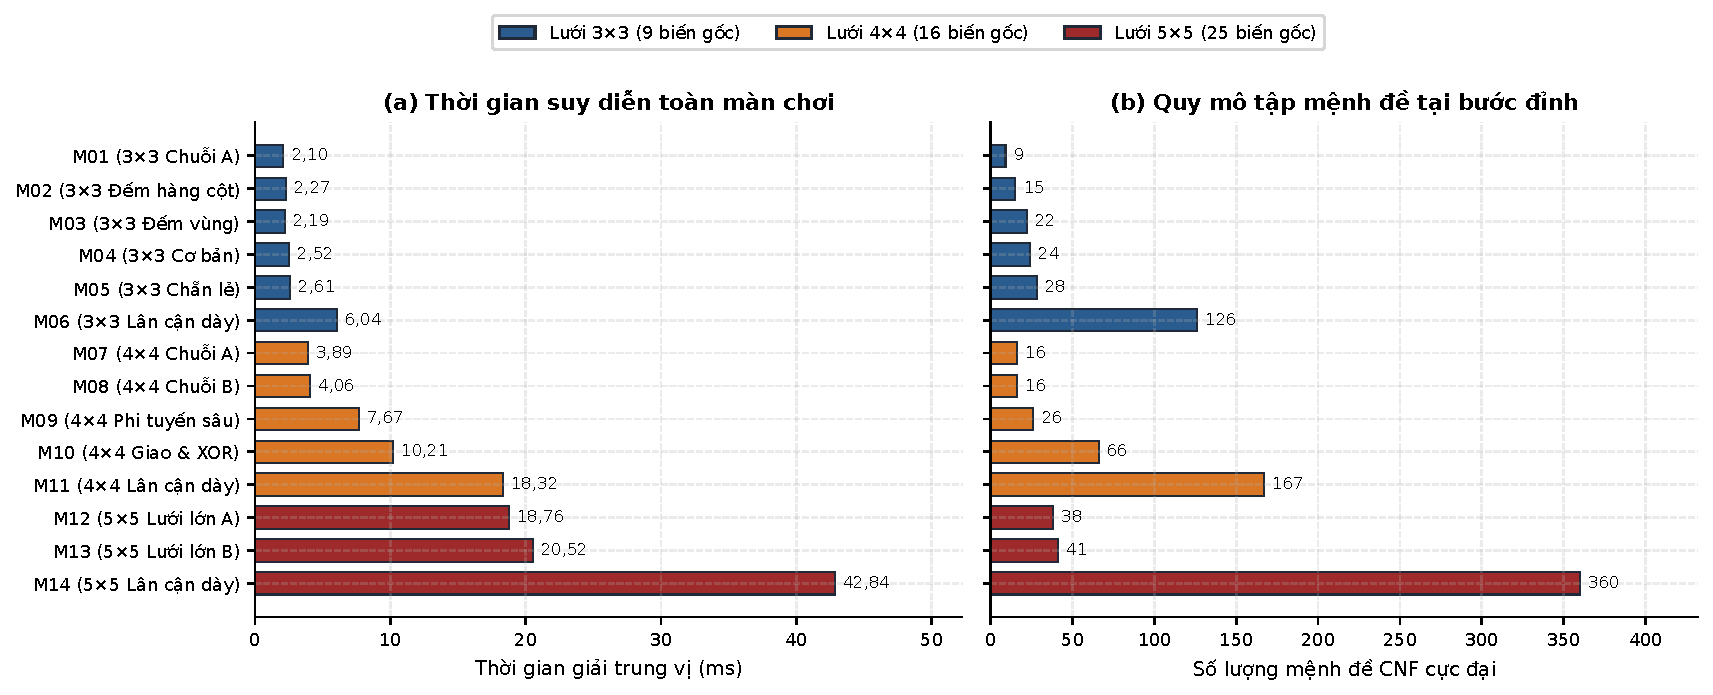
\includegraphics[width=0.98\textwidth]{images/charts/runtime_and_clauses.pdf}
    \caption{Đối sánh thời gian suy diễn trung vị (a) và số lượng mệnh đề CNF cực đại tại bước đỉnh (b) trên 14 màn chơi từ $3 \times 3$ đến $5 \times 5$}
    \label{fig:runtime_and_clauses}
\end{figure}

Đi sâu phân tích mối tương quan giữa cấu trúc mệnh đề và hành vi tìm kiếm bên trong bộ giải DPLL, số liệu thực nghiệm làm nổi bật hiệu lực áp đảo của cơ chế lan truyền mệnh đề đơn vị trên lớp bài toán suy diễn không đoán mò. Cụ thể, trên mười hai trong tổng số mười bốn màn chơi, số phép rẽ nhánh quyết định bằng không tuyệt đối, và trên toàn bộ mười bốn màn chơi không hề xuất hiện bất kỳ thao tác quay lui nào ($\text{Quay lui} = 0$). Hiện tượng này bắt nguồn từ bản chất toán học của câu đố: khi một ô thực sự bị ép buộc bởi các lời khai đang mở, việc tiêm giả định trái dấu vào cơ sở tri thức sẽ kích hoạt một thác rút gọn liên hoàn trên các mệnh đề bậc hai và bậc ba, làm bộc lộ mệnh đề rỗng ngay ở tầng gốc của thủ tục lan truyền mà không cần mở cây tìm kiếm. Ngay cả tại hai màn lân cận phức tạp $\text{M11}$ ($2$ quyết định) và $\text{M14}$ ($1$ quyết định), các phép chọn biến tự do này chỉ diễn ra ở nhánh kiểm tra khả thỏa của một ô chưa đủ dữ kiện để hoàn thiện nhanh mô hình chứng nhân và thành công ngay ở nhánh thử đầu tiên.

Bên cạnh đó, biểu đồ phân tán hai chiều tại Hình \ref{fig:regimes_scatter} cho thấy thời gian thực thi tổng thể không tăng đơn điệu thuần túy theo kích thước bàn cờ, mà phân tách rõ rệt thành \textbf{hai chế độ chi phí tính toán đối lập nhau}. Ở chế độ thứ nhất bị chi phối bởi khối lượng truy vấn và lan truyền (điển hình là hai màn $\text{M12}$ và $\text{M13}$ trên lưới $5 \times 5$), tập mệnh đề rất gọn nhẹ ($38$ đến $41$ mệnh đề), song các điểm mở khóa suy diễn lại thường nằm sâu ở các hàng cuối bàn cờ; do tác tử luôn quét tuần tự từ góc trái trên xuống dưới, mỗi bước phải thẩm định qua nhiều ô chưa xác định trước khi chạm tới ô ép buộc, đẩy tổng số lượt gọi SAT lên $228$ lần cùng $2.563$ phép lan truyền đơn vị và tiêu tốn $20{,}52\text{ ms}$. Trái ngược hoàn toàn, ở chế độ thứ hai bị chi phối bởi mật độ mệnh đề tổ hợp (điển hình là $\text{M06}$, $\text{M11}$ và đặc biệt là $\text{M14}$), tác tử chỉ cần $67$ truy vấn SAT và $870$ phép lan truyền (ít hơn gần ba lần so với $\text{M13}$), nhưng thời gian chạy lại tăng gấp đôi lên mức đỉnh $42{,}84\text{ ms}$. Nguyên nhân sâu xa nằm ở chỗ một lời khai đếm chính xác $4$ tội phạm trên vùng tám ô lân cận bên trong lưới đã sinh tới $\binom{8}{5} + \binom{8}{4} = 126$ mệnh đề, đẩy quy mô tập mệnh đề của $\text{M14}$ lên $360$ mệnh đề và làm gia tăng đáng kể chi phí duyệt danh sách mệnh đề bên trong từng chu kỳ lan truyền đơn vị.

\begin{figure}[H]
    \centering
    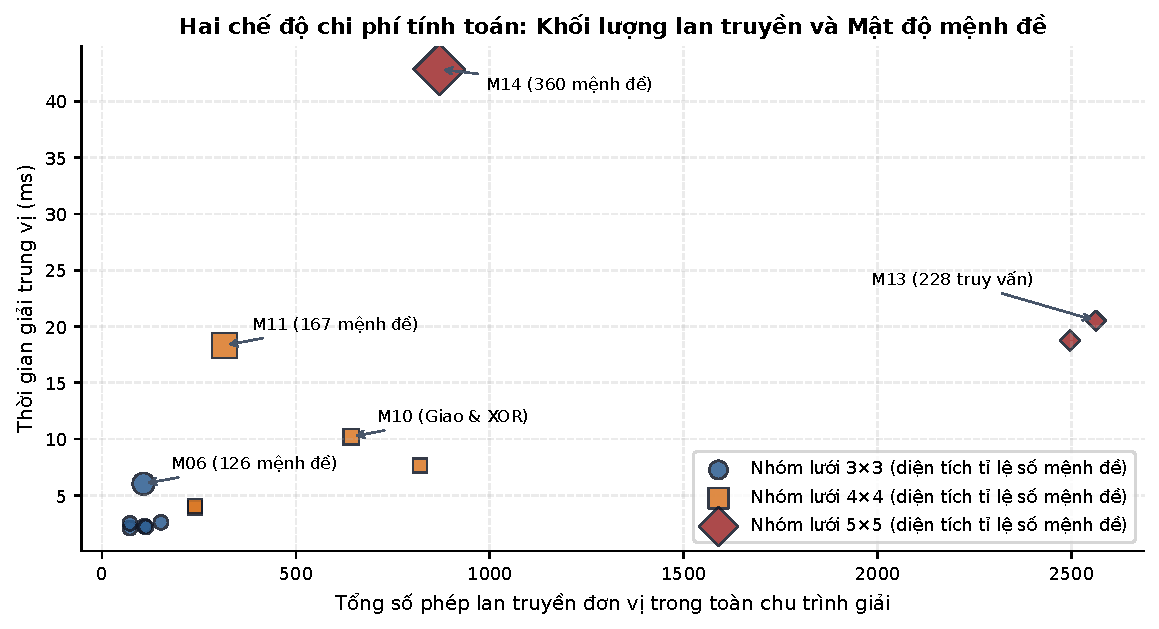
\includegraphics[width=0.78\textwidth]{images/charts/queries_vs_propagations.pdf}
    \caption{Sự phân hóa rõ nét giữa chế độ chi phối bởi mật độ mệnh đề tổ hợp (nhóm diện tích điểm lớn $\text{M06}, \text{M11}, \text{M14}$) và chế độ chi phối bởi khối lượng truy vấn ($\text{M12}, \text{M13}$)}
    \label{fig:regimes_scatter}
\end{figure}

\subsection{Đánh giá bóc tách bộ nhớ đệm}
\label{subsec:exp_ablation}
Nhằm kiểm chứng thực nghiệm giá trị của Mệnh đề 2 (Mục \ref{subsec:witness_cache}), nhóm thực hiện thí nghiệm bóc tách trên toàn bộ mười bốn màn chơi bằng cách đặt tác tử hoạt động ở hai chế độ đối chứng: tắt hoàn toàn bộ nhớ đệm mô hình chứng nhân (luôn thực hiện trọn vẹn cặp truy vấn giả định ngược cho từng ô) và bật bộ nhớ đệm mô hình chứng nhân theo từng bước. Hình \ref{fig:witness_ablation} và Bảng \ref{tab:ablation_summary} cho thấy việc tái sử dụng các mô hình thỏa mãn đã giúp cắt giảm tổng số lượt gọi DPLL trên toàn tập dữ liệu từ $930$ lượt xuống còn $863$ lượt (tiết kiệm $67$ lượt giải SAT, tương đương mức giảm $7{,}20\%$), đồng thời kéo giảm tổng số phép lan truyền đơn vị từ $9.493$ phép xuống $8.813$ phép (giảm $7{,}16\%$) mà vẫn giữ nguyên tuyệt đối thứ tự các bước suy diễn.

\begin{figure}[H]
    \centering
    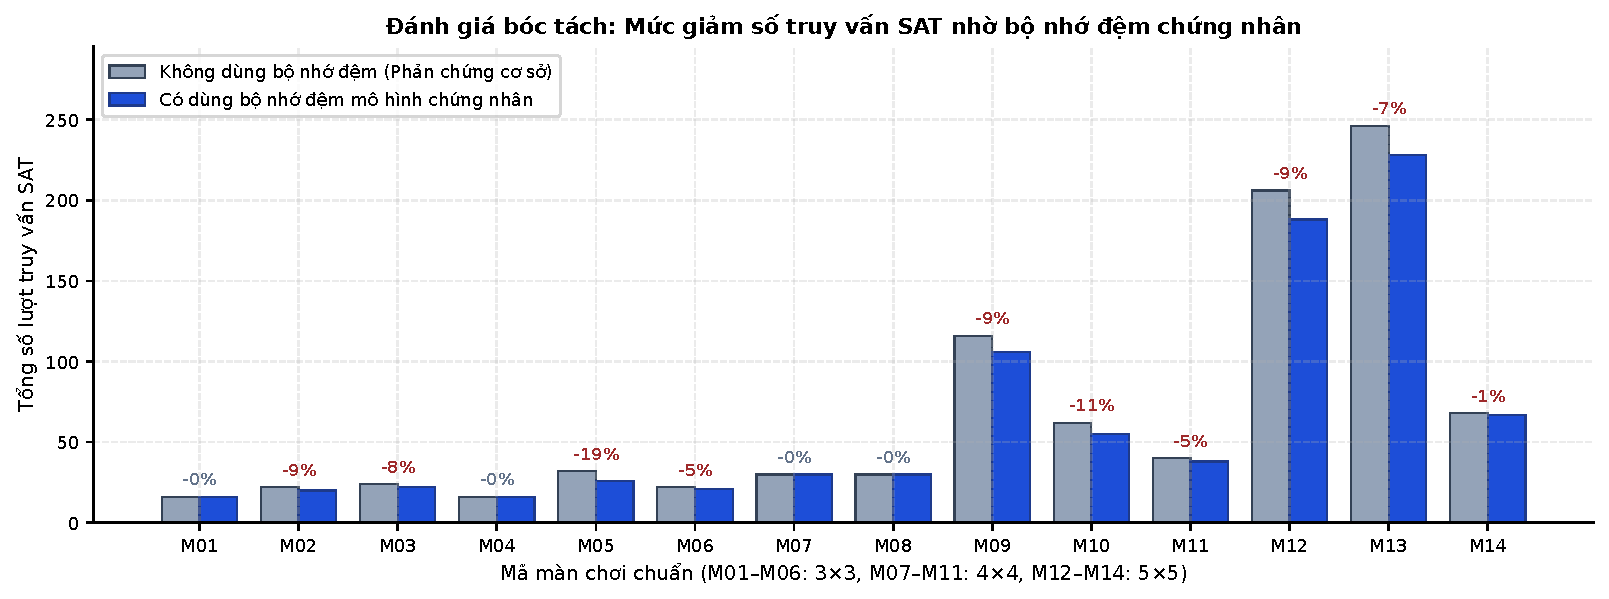
\includegraphics[width=0.96\textwidth]{images/charts/witness_cache_ablation.pdf}
    \caption{Kết quả thí nghiệm bóc tách số lượng truy vấn SAT khi tắt và bật bộ nhớ đệm mô hình chứng nhân trên 14 màn chơi}
    \label{fig:witness_ablation}
\end{figure}

\begin{table}[H]
\centering
\caption{Đối sánh định lượng hiệu quả của bộ nhớ đệm mô hình chứng nhân trên các màn chơi đại diện}
\label{tab:ablation_summary}
\resizebox{\textwidth}{!}{%
\begin{tabular}{l l c r r c r r c}
\toprule
\textbf{Mã} & \textbf{Đặc trưng tô-pô suy diễn} & \textbf{Lưới} & \textbf{Truy vấn (Tắt)} & \textbf{Truy vấn (Bật)} & \textbf{Tỷ lệ giảm} & \textbf{Lan truyền (Tắt)} & \textbf{Lan truyền (Bật)} & \textbf{Tỷ lệ giảm} \\
\midrule
M04 & Chuỗi thuận thứ tự quét hàng & $3\times3$ & 16  & 16  & $0{,}00\%$            & 72    & 72    & $0{,}00\%$ \\
M05 & Chẵn lẻ vùng nhảy cóc        & $3\times3$ & 32  & 26  & \textbf{$-18{,}75\%$} & 182   & 152   & \textbf{$-16{,}48\%$} \\
M07 & Chuỗi thuận thứ tự quét hàng & $4\times4$ & 30  & 30  & $0{,}00\%$            & 240   & 240   & $0{,}00\%$ \\
M09 & Suy diễn phi tuyến cuối bảng & $4\times4$ & 116 & 106 & $-8{,}62\%$           & 896   & 820   & $-8{,}48\%$ \\
M10 & Giao vùng kết hợp chuỗi XOR  & $4\times4$ & 62  & 55  & \textbf{$-11{,}29\%$} & 725   & 643   & \textbf{$-11{,}31\%$} \\
M12 & Mạng lưới rộng phi tuyến     & $5\times5$ & 206 & 188 & $-8{,}74\%$           & 2.735 & 2.496 & $-8{,}74\%$ \\
M13 & Mạng lưới rộng chuyên sâu    & $5\times5$ & 246 & 228 & $-7{,}32\%$           & 2.781 & 2.563 & $-7{,}84\%$ \\
\midrule
\multicolumn{2}{l}{\textbf{Tổng cộng toàn bộ 14 màn chơi}} & -- & \textbf{930} & \textbf{863} & \textbf{$-7{,}20\%$} & \textbf{9.493} & \textbf{8.813} & \textbf{$-7{,}16\%$} \\
\bottomrule
\end{tabular}%
}
\end{table}

Sự phân hóa tỷ lệ tiết kiệm giữa các màn chơi trong Bảng \ref{tab:ablation_summary} được giải thích rất nhất quán dưới góc độ tô-pô thứ tự suy diễn. Ở những màn chơi có lộ trình mở khóa thuận theo chiều quét ưu tiên hàng như $\text{M01}$, $\text{M04}$, $\text{M07}$ và $\text{M08}$, tại mọi bước lập luận, ngay ô chưa mở đầu tiên mà tác tử xét tới đã chính là ô bị ép buộc chân trị ($15\text{ bước} \times 2\text{ truy vấn} = 30\text{ truy vấn}$), do đó vòng lặp kết thúc bước ngay lập tức trước khi có bất kỳ ô chưa xác định nào được lưu chứng nhân ($0\%$ khác biệt). Ngược lại, trên những màn chơi có mạch suy diễn phi tuyến đòi hỏi nhảy vọt giữa các hàng cột xa nhau như $\text{M05}$, $\text{M09}$, $\text{M10}$, $\text{M12}$ và $\text{M13}$, ngay khi tác tử đi qua ô chưa xác định đầu tiên, hai mô hình thỏa mãn thu được sẽ phủ kín giá trị chân trị cho phần lớn các biến liên đới trên bàn cờ, giúp miễn trừ tức khắc một nửa số lượt gọi DPLL cho các ô tiếp theo và đem lại mức tiết kiệm lên tới $18{,}75\%$ trên màn $\text{M05}$ và $11{,}29\%$ trên màn $\text{M10}$.

\subsection{Phân tích độ mở rộng mệnh đề}
\label{subsec:exp_scaling}
Tiếp nối phân tích hiệu năng thời gian, Hình \ref{fig:encoding_scaling} khảo sát quy luật tăng trưởng số lượng mệnh đề CNF sinh ra khi kích thước vùng tác động $m = |R|$ mở rộng từ $2$ ô lên $16$ ô giữa ba chiến lược biên dịch: mã hóa chẵn lẻ trực tiếp từ bảng chân trị ($2^{m-1}$ mệnh đề, không biến phụ), mã hóa đếm lực lượng tổ hợp tại ngưỡng cân bằng $\lfloor m/2 \rfloor$ ($\binom{m}{\lfloor m/2 \rfloor + 1} + \binom{m}{\lceil m/2 \rceil + 1}$ mệnh đề, không biến phụ), và mã hóa chuỗi cổng tuyển loại trừ sử dụng $m - 2$ biến phụ Tseitin ($4m - 6$ mệnh đề). Ở phạm vi vùng rất hẹp $m \in \{3, 4\}$, cách mã hóa không biến phụ tỏ ra nhỉnh hơn đôi chút nhờ chỉ sinh từ $4$ đến $8$ mệnh đề ngắn. Thế nhưng ngay khi vượt qua ngưỡng $m \ge 6$, cả hai phương pháp không biến phụ đều bùng nổ theo tiệm cận hàm mũ Stirling $\binom{m}{m/2} \sim 2^m / \sqrt{\pi m / 2}$, trong khi đường biểu diễn của chuỗi cổng XOR biến phụ vẫn giữ độ dốc tuyến tính phẳng lặng. Tại mốc $m = 16$ (tương đương một lời khai bao trùm toàn bộ bàn cờ $4 \times 4$), bảng chân trị trực tiếp phát sinh tới $32.768$ mệnh đề và phép đếm tổ hợp phát sinh $22.880$ mệnh đề, trong khi mạch dây chuyền biến phụ chỉ cần vỏn vẹn $58$ mệnh đề bậc ba --- thu gọn dung lượng cơ sở tri thức tới $565$ lần.

\begin{figure}[H]
    \centering
    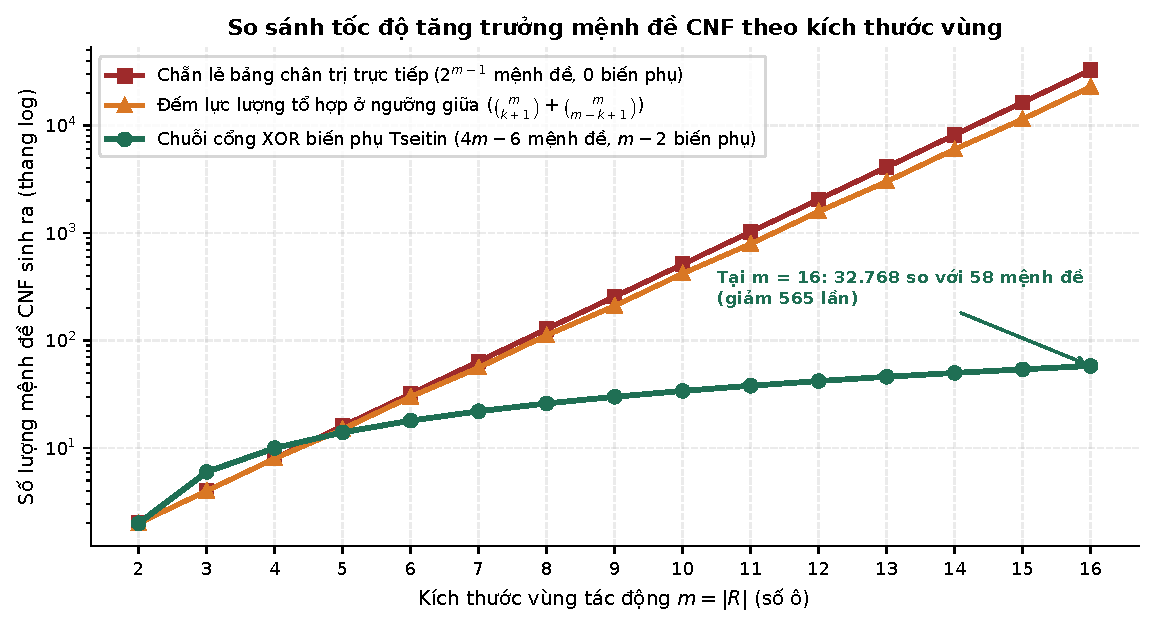
\includegraphics[width=0.78\textwidth]{images/charts/encoding_clause_scaling.pdf}
    \caption{Đối sánh tốc độ tăng trưởng mệnh đề CNF (trục tung logarit) giữa phương pháp hàm mũ/tổ hợp không biến phụ và chuỗi cổng XOR biến phụ tuyến tính}
    \label{fig:encoding_scaling}
\end{figure}

\subsection{Kịch bản biên và giới hạn hệ thống}
\label{subsec:exp_limitations}
Một báo cáo thực nghiệm khách quan không chỉ dừng lại ở các trường hợp thành công thuận lợi mà cần mổ xẻ thẳng thắn cách hệ thống phản ứng trước dữ liệu suy biến cũng như những điểm nghẽn kiến trúc khi đẩy bài toán tới cực hạn. Để phục vụ mục đích này, nhóm thiết kế bốn kịch bản đối kháng có kiểm soát (ký hiệu từ $\text{K01}$ đến $\text{K04}$) và ghi nhận kết quả thực thi thực tế trong Bảng \ref{tab:failure_stress}. Ở kịch bản thiếu dữ kiện $\text{K01}$ (chỉ cho biết hàng đầu tiên có đúng một tội phạm trong khi hai ô $\text{B1}$ và $\text{C1}$ hoàn toàn đối xứng nhau), quy trình kiểm định nghiệm duy nhất phát hiện ngay sự tồn tại của nghiệm thứ hai chỉ sau hai lượt giải, đồng thời chu trình giải tự động dừng lại an toàn ngay ở bước đầu tiên sau $14$ truy vấn kiểm tra mà không hề mạo hiểm đoán mò. Tương tự ở kịch bản dữ liệu hỏng $\text{K02}$ (một lời khai khẳng định $\text{B1}$ là tội phạm nhưng lời khai khác lại cấm toàn bộ hàng đầu tiên có tội phạm), tác tử lập tức phát hiện cơ sở tri thức vô nghiệm chỉ trong $0{,}11\text{ ms}$ và ngắt chu trình trước khi làm sai lệch trạng thái bàn cờ.

\begin{table}[H]
\centering
\caption{Kết quả kiểm thử các kịch bản suy biến có kiểm soát và bài toán vô nghiệm áp lực cao}
\label{tab:failure_stress}
\scriptsize
\setlength{\tabcolsep}{4.5pt}
\begin{tabularx}{\textwidth}{l >{\raggedright\arraybackslash}X r r r r r c}
\toprule
\textbf{Mã} & \textbf{Cấu trúc ràng buộc đối kháng} & \textbf{Mệnh đề} & \textbf{Nhánh} & \textbf{Lan truyền} & \textbf{Quay lui} & \textbf{Thời gian (ms)} & \textbf{Kết cục xử lý} \\
\midrule
K01 & Màn $3\times3$ khuyết thiếu dữ kiện khiến hai ô đối xứng hoàn toàn & 6  & 0     & 28    & 0     & 0,84  & Dừng an toàn (Đa nghiệm) \\
K02 & Màn $3\times3$ chứa hai lời khai trực tiếp phủ định lẫn nhau       & 5  & 0     & 2     & 0     & 0,11  & Ngắt an toàn (Mâu thuẫn) \\
K03 & Lưới $4\times4$ vô nghiệm đếm: 4 hàng có đúng 2 tội phạm nhưng 4 cột có tối đa 1 & 56 & 10    & 71    & 10    & 0,65  & Bác bỏ thành công \\
K04 & Lưới $4\times4$ vô nghiệm chẵn lẻ: 4 hàng tổng chẵn nhưng 3 cột tổng lẻ và 1 cột chẵn & 80 & \textbf{1.022} & \textbf{5.220} & \textbf{1.022} & \textbf{87,24} & Bác bỏ thành công \\
\bottomrule
\end{tabularx}
\end{table}

Đáng chú ý hơn cả là sự tương phản sâu sắc giữa hai bài toán vô nghiệm toàn cục trên lưới $4 \times 4$ ($\text{K03}$ và $\text{K04}$), qua đó phơi bày ba giới hạn kỹ thuật trung thực của hệ thống hiện tại. Giới hạn thứ nhất nằm ở \textbf{điểm mù phân giải của giải thuật DPLL thuần túy trước hệ phương trình tuyến tính trên trường hữu hạn $\mathbb{F}_2$} \cite{tseitin1983complexity,urquhart1987hard}: trong khi mâu thuẫn tổng lực lượng ở $\text{K03}$ ($8 \ne 4$) được DPLL bác bỏ dễ dàng chỉ sau $10$ nhánh quay lui ($0{,}65\text{ ms}$), thì mâu thuẫn chẵn lẻ toàn cục ở $\text{K04}$ (tổng bốn hàng chẵn bằng $0 \pmod 2$ đối chọi với tổng ba cột lẻ cộng một cột chẵn bằng $1 \pmod 2$) lại buộc bộ giải phải duyệt sâu tới $1.022$ quyết định rẽ nhánh, $5.220$ phép lan truyền và $1.022$ lần quay lui trong $87{,}24\text{ ms}$. Nguyên nhân là mỗi mệnh đề bậc ba của cổng XOR chỉ có thể kích hoạt lan truyền đơn vị khi đã biết trước hai trong ba biến; do không tích hợp phép khử Gauss--Jordan chuyên biệt \cite{soos2009extending}, DPLL buộc phải rẽ nhánh mũ trên cây tìm kiếm mới phát hiện ra tính vô nghiệm toàn cục. Giới hạn thứ hai là phép biên dịch đếm lực lượng hiện chưa sử dụng biến phụ bộ đếm tuần tự \cite{sinz2005towards}; dù rất nhanh trên các vùng $\le 8$ ô, nếu áp dụng cho một lời khai đếm $12$ tội phạm trên toàn mặt bàn $5 \times 5$ ($m = 25$), tổ hợp $\binom{25}{13} + \binom{25}{14}$ sẽ vượt ngưỡng chín triệu mệnh đề và gây tràn bộ nhớ. Cuối cùng, giới hạn thứ ba đến từ việc bộ giải được cài đặt trên ngôn ngữ thông dịch bậc cao với thao tác quét tuần tự danh sách mệnh đề và sao chép bảng gán khi rẽ nhánh thay vì cấu trúc hai con trỏ theo dõi (\textit{two-watched literals}) và học mệnh đề xung đột (\textit{CDCL}) \cite{silva1999grasp,moskewicz2001chaff}, khiến tốc độ xử lý sẽ suy giảm nếu mở rộng lên quy mô lưới lớn cỡ $10 \times 10$.

\section{Kết luận và hướng phát triển}
\label{sec:conclusion}

\subsection{Tổng kết kết quả}
Nhìn lại quá trình nghiên cứu và triển khai, đồ án đã xây dựng hoàn chỉnh giải pháp
tự động hóa suy diễn logic mệnh đề tuân thủ nguyên tắc không suy đoán trên trò chơi
suy luận trinh thám dạng lưới, kết nối liền mạch giữa nền tảng lý thuyết hình thức
với kỹ nghệ phần mềm và đồ họa tương tác ba chiều. Ở tầng biểu diễn tri thức, nhóm
đã thiết lập hệ thống ánh xạ biến song ánh phân tách rõ không gian biến gốc và biến
phụ, đồng thời hiện thực thành công bộ mã hóa dạng chuẩn hội tự động cho sáu họ lời
khai cốt lõi cùng hai mở rộng quan trọng là đại số vùng giao và mạch chẵn lẻ biến
phụ Tseitin tuyến tính giúp thu gọn số mệnh đề hàng trăm lần trên miền rộng (cụ thể
$565$ lần tại $m = 16$). Toàn bộ hệ thống công thức mã hóa này đã được kiểm chứng
tương đương ngữ nghĩa vét cạn trên hàng chục nghìn cấu hình chân trị độc lập, bảo
đảm tính đúng đắn toán học của tầng biểu diễn.

Tiếp nối tầng biểu diễn, nhóm đã tự cài đặt hoàn chỉnh bộ giải thỏa mãn mệnh đề
DPLL tất định hỗ trợ giả định đầu vào và lan truyền đơn vị đến điểm bất động, làm
bộ giải cốt lõi cho tác tử suy diễn bằng phản chứng. Đặc biệt, việc đề xuất và
chứng minh chặt chẽ cơ chế bộ nhớ đệm nghiệm mẫu giới hạn trong phạm vi từng bước
đã giúp hệ thống cắt giảm tới $18{,}75\%$ số lượt gọi bộ giải trên các màn chơi phi tuyến (trung bình $7{,}20\%$ trên toàn tập), trong khi quy trình mệnh
đề chặn cho phép xác thực tính duy nhất của nghiệm chỉ sau đúng hai lượt giải SAT.
Kết quả thực nghiệm trên tiến trình độc lập qua $14$ màn chơi chuẩn từ $3 \times 3$
đến $5 \times 5$ ghi nhận tỷ lệ giải thành công $100\%$ với thời gian trung vị tối
đa chỉ $42{,}84\text{ ms}$, song hành cùng không gian bàn điều tra ba chiều
\textit{Midnight Archive} mang lại phản hồi đóng dấu trực quan ngay trên từng thẻ
nghi phạm.

\subsection{Hướng phát triển}
Từ những phân tích khách quan về giới hạn hệ thống tại Chương
\ref{sec:experiments}, nhóm định hình bốn hướng nghiên cứu nâng cấp có tính khả thi
cao trong tương lai. Hướng ưu tiên hàng đầu là tái cấu trúc bộ giải mệnh đề theo
kiến trúc học mệnh đề hướng xung đột (\textit{CDCL}) kết hợp cơ chế theo dõi hai
literal (\textit{two-watched literals}) \cite{silva1999grasp,moskewicz2001chaff} và
chiến lược chọn biến dựa trên mức độ tham gia xung đột (như nhánh heuristic VSIDS),
qua đó giảm đáng kể chi phí quét lại các mệnh đề đã thỏa và thao tác sao chép trạng
thái khi quay lui. Song song với cải tiến bộ giải tổng quát, việc bổ sung cơ chế mã
hóa thích nghi cho các ràng buộc đếm số lượng (\textit{cardinality}) --- tự động
chuyển sang mạch bộ đếm tuần tự đa thức $O(m \cdot k)$ của Sinz
\cite{sinz2005towards} mỗi khi kích thước vùng vượt quá tám ô --- sẽ cho phép xử
lý hiệu quả các lời khai bao quát toàn bộ bàn cờ cỡ lớn mà tránh được sự bùng nổ
số mệnh đề.

Bên cạnh hiệu năng trên lưới rộng, để khắc phục hạn chế phân giải của DPLL trước hệ
ràng buộc XOR toàn cục như đã ghi nhận ở kịch bản kiểm thử khắc nghiệt $\text{K04}$,
bộ giải có thể được tích hợp thêm mô-đun đại số tuyến tính thực hiện phép khử
Gauss--Jordan trực tiếp trên ma trận hệ số trường $\mathbb{F}_2$ theo hướng tiếp
cận lai ghép hiện đại \cite{soos2009extending}. Cuối cùng, về mặt khả năng giải
thích trực quan hỗ trợ người học và người chơi, nhóm hướng tới việc khai thác kỹ
thuật trích xuất tập con không thỏa tối tiểu (\textit{Minimal Unsatisfiable
Subset}) từ vết chứng minh vô nghiệm của $KB_t \wedge \neg \ell^*$; khi đó, công cụ
gợi ý trên bàn điều tra ba chiều không những xác định chính xác nghi phạm kế tiếp
có thể chứng minh mà còn tự động tổng hợp được lời giải thích ngôn ngữ tự nhiên
ngắn gọn chỉ dẫn đúng hai hoặc ba lời khai then chốt dẫn tới kết luận ấy.

\section{Quản lý đồ án và phụ lục}
\label{sec:contribution}

\subsection{Kế hoạch triển khai}
Để bảo đảm tiến độ đồng đều và tránh tình trạng chờ đợi dây chuyền giữa bốn thành
viên trong nhóm, dự án được tổ chức theo phương pháp thiết kế đặc tả giao tiếp
(\textit{API contract}) trước khi cài đặt chi tiết, chia làm ba giai đoạn nối tiếp
nhau rõ ràng. Trong giai đoạn khởi đầu, toàn nhóm cùng phân tích đặc tả bài toán,
thống nhất mô hình dữ liệu cốt lõi, quy ước định dạng mệnh đề số nguyên và ranh
giới truyền nhận dữ liệu bất biến giữa bộ điều hành trò chơi với tác tử suy diễn.
Nhờ bộ khung giao tiếp chuẩn hóa này, sang giai đoạn phát triển trọng tâm, cả bốn
phân hệ lớn --- bao gồm môi trường quản lý trạng thái ẩn kèm bộ mã hóa CNF, bộ
giải thỏa mãn mệnh đề DPLL tự cài đặt, tác tử suy diễn phản chứng kèm bộ nhớ đệm
chứng nhân, và tầng dịch vụ API kết nối trực tiếp kèm bộ công cụ đo kiểm hiệu năng
(\textit{benchmark}) trên tiến trình độc lập --- đều được lập trình và kiểm thử đơn
vị song song trên các nhánh làm việc riêng biệt. Ở giai đoạn tích hợp và hoàn
thiện, các nhánh thành phần được rà soát chéo và hợp nhất thông qua hệ thống kiểm
thử hồi quy tự động gồm $290$ ca kiểm thử, trước khi nâng cấp không gian giao diện
ba chiều, tiến hành $42$ lượt đo đạc thực nghiệm chính thức và biên soạn báo cáo
tổng kết.

\subsection{Phân công nhiệm vụ}
Bảng \ref{tab:team_contributions} trình bày chi tiết khối lượng công việc thực tế
do từng thành viên đảm nhận (đối chiếu trung thực với lịch sử đóng góp trên kho
lưu trữ chung của nhóm) cùng mức độ hoàn thành nhiệm vụ được giao. Theo quy chế
đánh giá của học phần, tỷ lệ hoàn thành $100\%$ ở cả bốn thành viên xác nhận mỗi
cá nhân đều đã thực hiện đầy đủ, đúng hạn và đạt yêu cầu chất lượng phần việc
chuyên môn được phân công.

\begin{table}[htbp]
\centering
\caption{%
    Bảng phân công nhiệm vụ chuyên môn và tỷ lệ hoàn thành của các thành viên
    trong nhóm}
\label{tab:team_contributions}
\setstretch{1.08}
\scriptsize
\renewcommand{\arraystretch}{1.2}
\begin{tabularx}{\textwidth}{p{3.4cm} l >{\raggedright\arraybackslash}X c}
\toprule
\textbf{Họ và Tên} & \textbf{MSSV} & \textbf{Nội dung công việc đảm nhiệm thực tế} &
\textbf{Hoàn thành} \\
\midrule
\textbf{Nguyễn Phúc Khang}\newline \textit{(Trưởng nhóm)} & 24120068 &
Định hình kiến trúc phân tầng tổng thể, thiết kế mô hình dữ liệu cốt lõi và điều
phối rà soát hợp nhất các nhánh phát triển của nhóm. Xây dựng bộ quản lý trạng thái
ẩn, quy trình kiểm định tính trung thực lời khai, kho cơ sở dữ liệu $14$ màn chơi
chuẩn và bộ đánh giá ngữ nghĩa đối chứng độc lập. Nghiên cứu và hiện thực bộ mã
hóa tự động sang dạng chuẩn hội cho sáu họ manh mối cốt lõi cùng hai mở rộng giao
vùng hình học và mạch chẵn lẻ biến phụ Tseitin tuyến tính. Thiết kế không gian bàn
điều tra ba chiều \textit{Midnight Archive} với hiệu ứng ánh sáng vật lý, hiệu ứng
shader mưa đêm, con dấu đóng trực tiếp lên thẻ và tổng hợp biên tập báo cáo tổng
kết đồ án. & \textbf{100\%} \\
\midrule
\textbf{Phạm Minh Trọng} & 24120151 &
Thiết kế và hiện thực tầng dịch vụ API quản lý định danh phiên làm việc, đồng bộ số
hiệu phiên bản tương tranh lạc quan và kết nối luồng kiểm chứng phán quyết, gợi ý
cùng giải tự động từng bước. Xây dựng bộ công cụ đo kiểm hiệu năng chạy trên tiến
trình hệ điều hành độc lập với cơ chế áp đặt giới hạn thời gian cứng, thu thập chỉ
số đo đạc trên $14$ màn chơi và tự động tổng hợp dữ liệu thực nghiệm. Phát triển
hệ thống kiểm thử tích hợp đầu--cuối và rà soát đối chiếu số liệu thống kê trong
báo cáo. & \textbf{100\%} \\
\midrule
\textbf{Trần Nguyễn Anh Khoa} & 24120075 &
Nghiên cứu lý thuyết và hiện thực từ đầu bộ giải thỏa mãn mệnh đề DPLL tất định
thuần túy không sử dụng thư viện giải ngoài. Xây dựng cơ chế tiếp nhận giả định
tạm thời không làm biến đổi cơ sở tri thức, thủ tục lan truyền mệnh đề đơn vị lặp
đến điểm bất động, phát hiện xung đột mệnh đề rỗng sớm, chiến lược chọn biến rẽ
nhánh tất định kèm sao chép cô lập trạng thái quay lui và bộ đếm thống kê thực thi
chi tiết. Thiết kế bộ kiểm thử chuyên sâu cho bộ giải trên các công thức biên và
công thức bất khả thỏa lớn. & \textbf{100\%} \\
\midrule
\textbf{Bùi Nhật Bảo} & 24120167 &
Nghiên cứu và hiện thực tác tử suy diễn logic dựa trên nguyên lý chứng minh phản
chứng bốn trạng thái tuân thủ chặt chẽ quy tắc không suy đoán thiếu căn cứ. Đề xuất
ý tưởng, chứng minh tính đúng đắn và cài đặt cơ chế bộ nhớ đệm mô hình chứng nhân
theo từng bước suy diễn nhằm cắt giảm các lượt giải dư thừa. Xây dựng chu trình
giải tự động theo thứ tự ưu tiên hàng có ghi vết suy diễn đối soát từng bước, thuật
toán sinh gợi ý an toàn từ dữ kiện công khai và quy trình kiểm định nghiệm duy nhất
sử dụng mệnh đề chặn. & \textbf{100\%} \\
\bottomrule
\end{tabularx}
\end{table}

\subsection{Tài nguyên dự án}
Toàn bộ mã nguồn của hệ thống, tập dữ liệu $14$ màn chơi chuẩn, bộ $290$ kịch bản
kiểm thử tự động, công cụ tái lập thực nghiệm cùng video minh họa toàn bộ luồng
hoạt động trên không gian bàn điều tra ba chiều (quay ở độ phân giải cao
$1600 \times 900$ tốc độ $30$ khung hình/giây, trình diễn đầy đủ thao tác quan sát
cảnh ba chiều, lọc vùng manh mối, phản hồi đóng dấu từ chối trực tiếp lên mặt thẻ
khi kết luận sớm, sử dụng gợi ý và giải tự động tới khi khép lại vụ án) được lưu
trữ công khai tại kho mã nguồn trực tuyến của nhóm:
\url{https://github.com/khang1108/griductive}.

\subsection{Tuyên bố sử dụng trí tuệ nhân tạo}
\label{subsec:ai_appendix}
Tuân thủ nguyên tắc liêm chính học thuật và yêu cầu minh bạch tại Mục 4.6 của đề
cương đồ án, nhóm xin khai báo cụ thể phạm vi ứng dụng các mô hình ngôn ngữ lớn
trong quá trình thực hiện dự án. Trong suốt chu kỳ phát triển, công cụ trợ lý AI
chỉ được sử dụng như một phương tiện hỗ trợ kỹ thuật ở các khâu phụ trợ gồm: tham
khảo cách tổ chức ánh sáng vật lý, vật liệu bề mặt gỗ và kỹ thuật viết chương trình
shader cửa sổ mưa đêm trong môi trường đồ họa ba chiều trên trình duyệt; gợi ý mở
rộng thêm các kịch bản kiểm thử biên tự động để nâng cao độ bao phủ kiểm thử phần
mềm; đồng thời hỗ trợ rà soát lỗi chính tả, căn chỉnh bố cục bảng biểu và sơ đồ
khối trong quá trình chế bản tài liệu \LaTeX.

Để làm rõ cách thức tương tác có kiểm soát của nhóm với công cụ hỗ trợ, dưới đây
là ba yêu cầu truy vấn (\textit{prompt}) tiêu biểu đại diện cho các tình huống tra
cứu kỹ thuật thực tế trong dự án:
\begin{softbox}
\textbf{Prompt mẫu 1 (Kiểm chứng chéo tính tương đương ngữ nghĩa của bộ mã hóa):}
\textit{``Hãy đề xuất kịch bản kiểm thử vét cạn toàn bộ phép gán chân trị trên lưới
$3 \times 3$ và $4 \times 4$ để đối chiếu tập cấu hình thỏa mãn theo định nghĩa ngữ
nghĩa gốc với kết quả khả thỏa của công thức chuẩn hội sau khi mã hóa, đặc biệt chú
ý các trường hợp biên của ràng buộc chẵn lẻ dùng biến phụ Tseitin và vùng giao hình
học.''}\\[6pt]
\textbf{Prompt mẫu 2 (Thiết kế hiệu ứng phản hồi trực quan ba chiều tối giản):}
\textit{``Làm thế nào để thiết kế hoạt ảnh một con dấu cao su nghiêng dập trực
tiếp lên bề mặt thẻ nghi phạm trong không gian ba chiều rồi từ từ mờ dần khi người
chơi đưa ra phán quyết chưa đủ cơ sở chứng minh, nhằm thay thế các hộp thoại thông
báo gây rối mắt trên màn hình?''}\\[6pt]
\textbf{Prompt mẫu 3 (Chế bản học thuật trong \LaTeX):} \textit{``Hướng dẫn cách
căn chỉnh sơ đồ kiến trúc phân tầng bằng thư viện vẽ vector trong \LaTeX{} để thể
hiện rõ luồng dữ liệu một chiều chỉ trích xuất trạng thái công khai từ bộ điều hành
trò chơi sang tầng tác tử suy diễn.''}
\end{softbox}

Nhóm xin cam kết và chịu trách nhiệm rằng toàn bộ phần mô hình hóa toán học biến
mệnh đề, các phép biến đổi đại số tương đương sang dạng chuẩn hội, thuật toán giải
thỏa mãn mệnh đề DPLL tự cài đặt, định lý phản chứng cùng cơ chế bộ nhớ đệm mô
hình chứng nhân của tác tử suy diễn, cũng như toàn bộ số liệu thực nghiệm thu thập
từ $42$ lượt đo đạc độc lập và nội dung phân tích học thuật trong báo cáo này đều
do các thành viên trong nhóm trực tiếp nghiên cứu, thiết kế, kiểm chứng chéo và
biên soạn.


\newpage
\nocite{*}
\bibliographystyle{IEEEtran}
\bibliography{ref}

\end{document}
